\documentclass[a4paper]{report}
\usepackage{thuvien}
\usepackage{a4wide,amssymb,epsfig,latexsym,multicol,array,hhline,fancyhdr}
\usepackage{ragged2e}
\usepackage{booktabs, makecell, tabularx}
\AtBeginDocument{\addtocontents{toc}{\protect\thispagestyle{empty}}}
\hypersetup{
    colorlinks,
    citecolor=green,
    filecolor=red,
    linkcolor=black,
    urlcolor=blue
}
\PassOptionsToPackage{hyphens}{url}
\usepackage{breakurl}

\newcommand{\monhoc}{Đồ án kỹ thuật máy tính}
\newcommand{\mamon}{CO2018}
\newcommand{\nienkhoa}{2018-2019}
\setlength{\headheight}{40pt}

\fancyhead{} % clear all header fields
\fancyhead[L]{
 \begin{tabular}{rl}
    \begin{picture}(25,15)(0,0)
    \put(0,-8){
\includegraphics[width=8mm, height=8mm]{../images/logo/bklogo.png}}
   \end{picture}&
	\begin{tabular}{l}
		\textbf{\bf \ttfamily Đại Học Bách Khoa Tp.Hồ Chí Minh}\\
		\textbf{\bf \ttfamily Khoa Khoa học và Kỹ thuật máy tính}
	\end{tabular} 	
 \end{tabular}
}
\fancyhead[R]{
	\begin{tabular}{l}
		\textbf{\bf \ttfamily \monhoc}\\
		\textbf{\bf \ttfamily Niên khóa 2018-2019} 
	\end{tabular}  }
\fancyfoot{} % clear all footer fields
\fancyfoot[L]{\scriptsize \ttfamily \rightmark}
\fancyfoot[R]{\scriptsize \ttfamily Trang {\thepage}/\pageref{LastPage}}
\renewcommand{\headrulewidth}{0.3pt}
\renewcommand{\footrulewidth}{0.3pt}

% Redefine the plain page style
\fancypagestyle{plain}{%
  \fancyhf{}%
  \fancyfoot[L]{\scriptsize \ttfamily \rightmark}
  \fancyfoot[R]{\scriptsize \ttfamily Trang {\thepage}/\pageref{LastPage}}
  \renewcommand{\headrulewidth}{0pt}% Line at the header invisible
  \renewcommand{\footrulewidth}{0.3pt}% Line at the footer visible
}
%dont ever touch this 
\makeatletter
\renewcommand\listoftables{%
    \subsection{\listtablename}%
    \@mkboth{\MakeUppercase\listtablename}%
        {\MakeUppercase\listtablename}%
    \@starttoc{lot}%
}
\renewcommand\listoffigures{%
    \subsection{\listfigurename}%
    \@mkboth{\MakeUppercase\listfigurename}%
        {\MakeUppercase\listfigurename}%
    \@starttoc{lof}%
}
\makeatother
%i have warned you
\lstnewenvironment{lst}
  {%
   \mdframed[backgroundcolor=black!10, linecolor=none]%
   \lstset{
   				language = bash,
   				basicstyle=\fontsize{9}{11}
  				showstringspaces=false,
  				stepnumber=1,
  				breaklines=true,
  				postbreak=\mbox{\textcolor{blue}{$\hookrightarrow$}\space},
			}
  }
  {\endmdframed}
  
\usepackage{xcolor}
\definecolor{dkgreen}{rgb}{0,0.6,0}
\definecolor{dred}{rgb}{0.545,0,0}
\definecolor{dblue}{rgb}{0,0,0.545}
\definecolor{lgrey}{rgb}{0.9,0.9,0.9}
\definecolor{gray}{rgb}{0.4,0.4,0.4}
\definecolor{darkblue}{rgb}{0.0,0.0,0.6}
\lstdefinelanguage{cpp}{
      backgroundcolor=\color{lgrey},  
      basicstyle=\footnotesize \ttfamily \color{black} \bfseries,   
      breakatwhitespace=false,       
      breaklines=true,               
      captionpos=b,                   
      commentstyle=\color{dkgreen},   
      deletekeywords={...},          
      escapeinside={\%*}{*)},                  
      frame=single,                  
      language=C++,                
      keywordstyle=\color{dblue},  
      morekeywords={BRIEFDescriptorConfig,string,TiXmlNode,DetectorDescriptorConfigContainer,istringstream,cerr,exit}, 
      identifierstyle=\color{black},
      stringstyle=\color{blue},      
      numbers=left,                 
      numbersep=5pt,                  
      numberstyle=\tiny\color{black}, 
      rulecolor=\color{black},        
      showspaces=false,               
      showstringspaces=false,        
      showtabs=false,                
      stepnumber=1,                   
      tabsize=5,                     
      %title=\lstname,                 
    }
%%%%%%%%%%%%%%%%%%%%%%%%%%%%%%%%%%%%%%%%%%%%%%%%%%%%%%%%%
%%%%%%%%%%%%%%%%%%%%%%%%%%%%%%%%%%%%%%%%%%%%%%%%%%%%%%%%%
%%%%%%%%%%%%%%%%%%%%%%%%%%%%%%%%%%%%%%%%%%%%%%%%%%%%%%%%%

\begin{document}
\begin{titlepage}
\begin{center}
\textbf{ĐẠI HỌC QUỐC GIA THÀNH PHỐ HỒ CHÍ MINH \\
TRƯỜNG ĐẠI HỌC BÁCH KHOA \\
KHOA KHOA HỌC - KỸ THUẬT MÁY TÍNH }
\vspace{1cm}

\begin{figure}[h!]
\begin{center}

\includegraphics[width=3cm]{../images/logo/bklogo.png}
\end{center}
\end{figure}

\vspace{1cm}

\begin{tabular}{c}
\multicolumn{1}{l}{\textbf{{\Large Môn học: \monhoc}}}\\
\\
\hline
\\
\multicolumn{1}{l}{\textbf{{\Large Đề tài:}}}\\
\\
\textbf{{\Huge Nhận diện khuôn mặt }}\\
\textbf{{\Huge sử dụng trong phòng thí nghiệm}}\\
\\
\hline
\end{tabular}
\end{center}
\vspace{3cm}

\begin{table}[h]
\begin{tabular}{rrl}
\vspace*{1em}
\hspace{5 cm} & GVHD: & PGS.TS Trần Ngọc Thịnh\\
 & Sinh viên: & Nguyễn Bảo Khương - 1511632 \\
& & Hồ Quảng Nam - 1512065\\
& & Nguyễn Hoài Thương - 1512990\\
\end{tabular}
\end{table}
\vspace*{\fill}
\begin{center}
{\footnotesize TP. Hồ Chí Minh, \today}
\end{center}
\end{titlepage}
%%%%%%%%%%%%%%%%%%%%%%%%%%%%%%%%%%
\newpage
\tableofcontents
\thispagestyle{empty}
%%%%%%%%%%%%%%%%%%%%%%%%%%%%%%%%%%
\newpage

\setlength{\parskip}{0.5em}
\pagestyle{fancy}

\chapter{Giới thiệu}
\section{Đặt vấn đề}
Hơn ba thập kỉ qua, nhận dạng khuôn mặt đã trở thành một lĩnh vực nóng hổi trong ngành học liên quan đến Computer Vision (thị giác máy tính), Neuroscience (Khoa học thần kinh) và Biometrics (Sinh trắc học). 
\par\noindent
Nhận diện khuôn mặt sử dụng để xác thực người, đó là cách đơn giản nhất mà con người sử dụng. "Mỗi người có những đặc điểm riêng không chia sẻ với người khác" (Umer et al., 2015). Mặc dù còn nhiều tranh cãi, nó vẫn là một kĩ thuật có nhiều lợi điểm hơn một vài kĩ thuật nhận diện sinh trắc học khác để nhận biết sự xuất hiện của một người trong một khu vực nhất định.
\par\noindent
Để tạo ra một hệ thống nhận diện đủ độ tin cậy, cần phải có một tập cơ sở dữ liệu về khuôn mặt (database of facial images), một giải thuật phù hợp và một quy trình test hợp lí để đánh giá hệ thống. Trong thời đại công nghiệp 4.0 đòi hỏi các vấn đề được giải quyết bằng các giải pháp khoa học kĩ thuật, kỹ thuật nhận diện khuôn mặt cần phải được nghiên cứu và phát triển hơn nữa. 
\par\noindent
Nhận diện khuôn mặt có những lợi ích trong áp dụng thực tiễn không thể chối cãi và rất dễ dàng nhận thấy, một số ứng dụng tiêu biểu đó là nhận dạng người trong các cơ quan, chính phủ (ID quốc gia, hộ chiếu, giấy phép,..) và xác minh danh tính tự động (kiểm soát biên giới). Giúp đỡ các cơ quan điều tra trong tìm kiếm tội phạm, khủng bố, ... Woodward Jr và các cộng sự năm 2003 đã nói "Lĩnh vực nghiên cứu này hứa hẹn sẽ phát triển hơn và được triển khai nhiều hơn trong an ninh và giám sát, cũng như trong các thiết bị cá nhân như máy ảnh, điện thoại, máy tính xách tay.
\section{Mục tiêu đề tài}
Có thể thấy rằng, việc nhận diện khuôn mặt đang là một lĩnh vực rất cần sự quan tâm trong thời đại công nghiệp 4.0 hiện nay. Do đó, cùng với sự thích thú và ham học hỏi trong lĩnh vực học máy, mong muốn áp dụng những công cụ đó vào thực tiễn, nhóm chúng tôi đã thực hiện đề tài về nhận diện khuôn mặt sử dụng trong phòng thí nghiệm bằng phương pháp học máy. Do giới hạn về phạm vi cũng như kiến thức chuyên môn. Đề tài tập trung thực hiện các mục tiêu sau:
\begin{enumerate}
\item Tìm hiểu về xử lí ảnh trong Computer Vision
\item Tìm hiểu về học máy (Machine Learning)
\item Tìm hiểu về Face Detection
\item Tìm hiểu về Face Regconition
\item Xây dựng một chương trình nhận diện khuôn mặt bằng code C/C++
\item Chạy chương trình trên Zedboard để nhận diện khuôn mặt thông qua camera
\item Đánh giá hệ thống và đề xuất cải tiến
\end{enumerate}
\section{Ý nghĩa đề tài}
Về chuyên môn: Đề tài có ý nghĩa như nền tảng cho cả nhóm thấy được cách xây dựng một ứng dụng trong thực tế áp dụng kiến thức của thời đại mới, sử dụng machine learning. Đồng thời áp dụng được ứng dụng đó xuống zedboard, một thiết bị hỗ trợ lập trình trên cả ARM và FPGA. Cho ta thêm cơ hội tìm hiểu các giải thuật để giải quyết vấn đè về nhận diện khuôn mặt, nhận diện vật thể và xử lí hình ảnh, làm việc với một hệ thống không quen thuộc, với các phần mềm hỗ trợ mới như Vivado, Xilinx SDK, ...
\par\noindent
Về thực tiễn: Là cơ sở để thấy được rằng có thể sử dụng zedboard để nhận diện khuôn mặt nếu nó được kết nối với camera sử dụng trong phòng thí nghiệm, với việc cải thiện độ chính xác và tốc độ của giải thuật, việc ứng dụng nó vào trong thực tế là điều dễ dàng.
\section{Hạn chế}
Do nhóm sử dụng phương án dùng công cụ chuyển code C sang FPGA nên có thể không hiểu hết cũng như không tận dụng hết được sức mạnh tính toán của nó.
\par\noindent
Việc sử dụng các thư viện xử lí hình ảnh sẽ đòi hỏi kiến thức và trình độ chuyên môn cao nếu muốn áp dụng chúng xuống dưới một thiết bị phần cứng như zedboard. Vì vậy sẽ tốn rất nhiều thời gian nếu muốn thực hiện một cách hoàn chỉnh.
\chapter{Kiến thức nền tảng}
\section{Cơ sở lý thuyết}
\subsection{Machine Learning}
Machine Learning là một lĩnh vực trong AI (trí tuệ nhân tạo), nó có khả năng tự học hỏi dựa trên dữ liệu đưa vào mà không cần phải được lập trình cụ thể mục đích chính của nó là tìm được một model có thể best fit được các dữ kiện cho trước để từ đó có thể dự đoán được kết quả của các dữ kiện tương lai.
\par\noindent
Có 2 định nghĩa được đưa ra về học máy. Arthur Samuel (1959) định nghĩa là: "một lĩnh vực học cho phép máy tính có khả năng học mà không cần phải lập trình trực tiếp". Đây là cách định nghĩa cũ và không chính thức. Tom Mitchell (1998) cũng đưa ra một định nghĩa \cite{bib1} : "Một chương trình được gọi là đã học từ kinh nghiệm $E$ từ các tác vụ $T$ mà nó tin tưởng, có hiệu suất được đánh giá là P, nếu hiệu suất của nó với các tác vụ trong T, được gọi là P cải thiện với kinh nghiệm E."
\par\noindent
Việc áp dụng học máy là hết sức quan trọng trong nhận diện khuôn mặt, khi ta không chỉ cần 1 mà đến 2 tác vụ từ kết quả của học máy, đó là Face Detection và Face Regconition. Vậy, ta cần áp dụng kiến thức của học máy cho việc xây dựng 2 model
\par\noindent
\begin{itemize}
\item Model nhận biết mặt người cho phép ta xác định được bao nhiêu khuôn mặt xuất hiện trong ảnh cũng như nhận biết đó là khuôn mặt của một người.
\item Model được xây dựng từ tập dữ liệu đầu vào để xác định được chủ nhân của khuôn mặt đó là ai.
\end{itemize}
\subsection{Image Processing}
Máy tính không nhìn có mắt, nó nhìn sự vật thông qua chiếc camera và nó nhìn những khung hình là những ma trận số (từ 0-255). Chúng ta có thể chia các bức ảnh ở dạng trắng-đen(grayscale) hoặc ảnh màu (color).
\par\noindent
\subsection*{Ảnh đen trắng}
Đầu tiên chúng ta nói về ảnh đen trắng (grayscale), mỗi pixel đại diện cho độ sáng của điểm ảnh đó (với 255 là sáng nhất), như trong ví dụ ở hình \ref{imgcat} và ma trận mà máy tính nhìn thấy ở hình \ref{imgmatrix}
\begin{figure}[H]
\centering
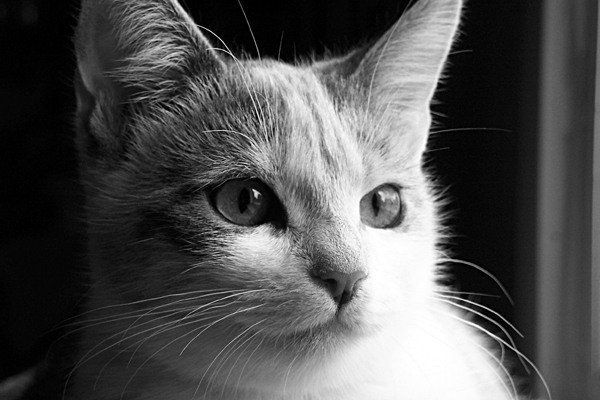
\includegraphics[scale=.4]{../images/fig/imgcat.jpg}
\caption{Ví dụ ảnh đen-trắng}
\label{imgcat}
\end{figure}
%
\begin{figure}[H]
\centering
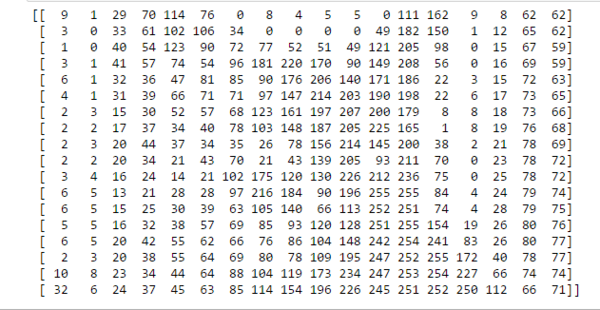
\includegraphics[scale=.4]{../images/fig/matrix.png}
\caption{Ma trận ảnh đen-trắng}
\label{imgmatrix}
\end{figure}
\noindent
Không như con người, máy tính nhìn hình ảnh dưới dạng ma trận 2 chiều. Một bức ảnh $1300*700px$ là bức ảnh có $1300$ điểm ảnh ngang và $700$ điểm ảnh dọc (một điểm ảnh ứng với một phần tử trong ma trận 2 chiều). Như vậy có tổng cộng $910,000$ ($1300*700$) pixels. Mỗi phần tử thể hiện độ sáng của điểm ảnh tại đó. Giá trị 0 biểu diễn giá trị đen (black) và 255 biểu diễn màu trắng (white). 
\subsection*{Ảnh màu}
Trong ảnh đen trắng, mỗi giá trị của điểm ảnh chỉ biểu diễn cường độ sáng của nó, còn gọi là ảnh chỉ có một kênh (channel). Trong ảnh màu, ảnh có đến 3 kênh: R(Red), B(Blue), G(Green). Một camera số chuẩn sẽ tạo ra ảnh có 3 kênh màu này (RGB).
%
\begin{figure}[H]
\centering
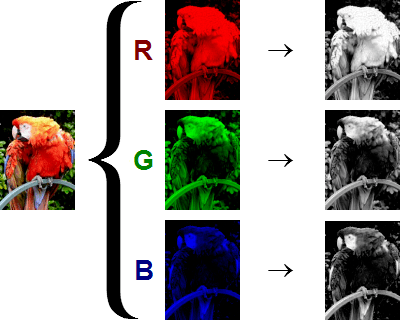
\includegraphics[scale=.6]{../images/fig/color.png}
\caption{Minh họa về các kênh màu của ảnh}
\label{fig:color}
\end{figure}
%
\noindent
Như ta có thể thấy trên hình \ref{fig:color}, hình ảnh được hợp thành từ 3 kênh red, green và blue. Không giống như ảnh trắng đen, ảnh màu được máy tính nhìn dưới ma trận 3 chiều, với chiều thứ 3 là số kênh, mỗi kênh sẽ là một ma trận 2 chiều, như vậy chúng ta có 3 ma trận ứng với mỗi kênh Red, Green và Blue xếp chồng lên nhau tạo thành ma trận 3 chiều. Mỗi điểm ảnh trong mỗi ma trận có giá trị từ $0-255$ tương ứng với mức red, blue hay green của nó tùy vào nó đang ở ma trận ứng với kênh nào.
\begin{figure}[H]
\centering
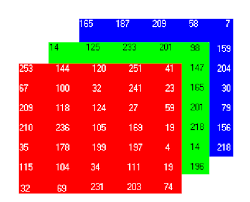
\includegraphics[scale=.6]{../images/fig/matrix2.png}
\caption{Ma trận RGB}
\label{fig:matrix2}
\end{figure}
\subsection*{Image Processing}
Xử lí ảnh cũng chính là bước tiền xử lí trong nhận diện khuôn mặt, hay còn gọi là low-level process, nó có trách nhiệm quan trọng trong việc tạo ra được input "chuẩn" cho bộ xử lí nhận diện, các công việc thường được làm ở giai đoạn này là:
\begin{itemize}
\item Giảm nhiễu
\item Điều chỉnh độ tương phản
\item Điều chỉnh độ sắc nét
\end{itemize}
%
\begin{figure}[H]
\centering
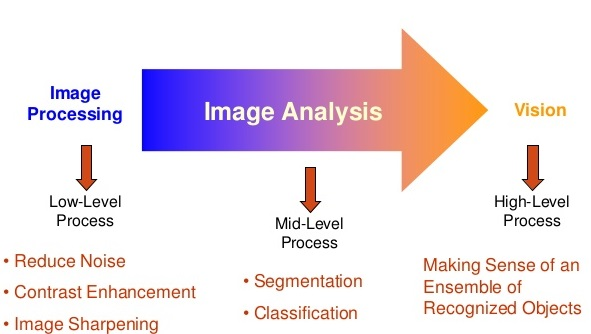
\includegraphics[scale=.5]{../images/fig/imgpro.jpg}
\caption{Minh họa quy trình xử lí ảnh}
\label{fig:imgpro}
\end{figure}
%
\subsection{Face Detection}
Face Detection, hay phát hiện khuôn mặt trong các bức ảnh số là bước đầu tiên để thực hiện việc nhận dạng hoặc thậm chí là dùng để tạo ra tập dữ liệu train đầu vào. Lẽ dĩ nhiên ta không thể nhận dạng được nếu ta còn không xác định được đó có phải mặt người hay không. 
%
\begin{figure}[H]
\centering
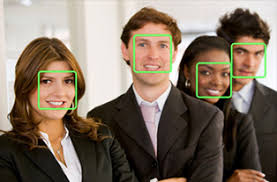
\includegraphics[scale=.5]{../images/fig/fdetect.jpg}
\caption{Minh họa cho công cụ phát hiện khuôn mặt}
\label{fig:imgpro}
\end{figure}
%
\noindent
Face Detection là một nhánh nhỏ trong lĩnh vực nhận diện vật thể. Các giải thuật của nó tập trung vào phát hiện mặt trước của khuôn mặt con người. Các giải thuật đáng tin cậy trong việc này thường được dựa vào thuật toán di truyền (genetic algorithm)và kỹ thuật eigen-face\cite{genetic}(the eigen-face technique)\cite{eigen}
\begin{itemize}
\item[-] Đầu tiên, các vùng mắt người có thể được phát hiện bằng cách kiểm tra tất cả các vùng thung lũng trong hình ảnh trắng đen. Sau đó, thuật toán di truyền được sử dụng để tạo ra tất cả các vùng khuôn mặt có thể bao gồm lông mày, mống mắt, lỗ mũi và khóe miệng.
\item[-]  Kế tiếp, mỗi "ứng viên" cho khuôn mặt sẽ qua các bước chuẩn hóa để giảm các hiệu ứng như ánh sáng không đều, ảnh bị nhòe v.v. Hình ảnh tốt nhất của các ứng viên sẽ thông qua các bước kiểm tra tiếp theo theo điều kiện của giải thuật. Tất cả ứng viên với giá trị thích hợp nhất sẽ được xác định là mặt người.
\end{itemize}
%
\subsection{Face Regconition}
Face recognition hay nhận diện khuôn mặt thường trải qua các bước như:
\begin{enumerate}
\item Preprocessing - Tiền xử lí: đây là giai đoạn hình ảnh lấy được từ camera sẽ được xử lí (giảm chiều, chuyển sang trắng đen, tăng độ tương phản,...) nhằm tạo ra input tốt nhất cho các bộ xử lí ở phần sau
\item Face detection: Sau khi đã có một bức ảnh đạt chuẩn từ bước tiền xử lí, bộ nhận diện khuôn mặt phải cố định được vùng chứa khuôn mặt (localize), thường ở bước này sẽ cắt vùng chứa khuôn mặt để sử dụng cho bước tiếp theo
\item Face normalization: chuẩn hóa lại vùng chứa khuôn mặt để có khuôn mặt tốt nhất cho việc nhận diện (xoay chiều ảnh cho đúng vị trí mặt nếu nghiêng, tăng giảm kích thước ảnh cho phù hợp,...)
\item Feature extraction: Chiết xuất các features cần thiết cho model đã được train trước đó
\item Feature matching: Đem các feature đó cho giải thuật so sánh xem nó phù hợp với dữ liệu trong tập dữ liệu không và đưa ra kết quả cuối cùng về nhân dạng của người trong ảnh
\end{enumerate}
\begin{figure}[H]
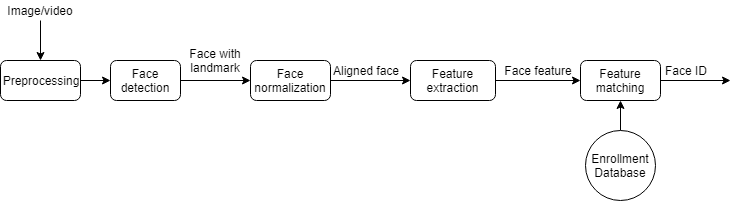
\includegraphics[width=\textwidth]{../images/fig/hinh3.png}
\caption{Quy trình nhận diện khuôn mặt}
\label{fig:hinh3}
\end{figure}
\noindent
Kết hợp với machine learning, ta có toàn bộ quy trình tổng quát cần phải thực hiện để nhận diện khuôn mặt như sau:
%
\begin{figure}[H]
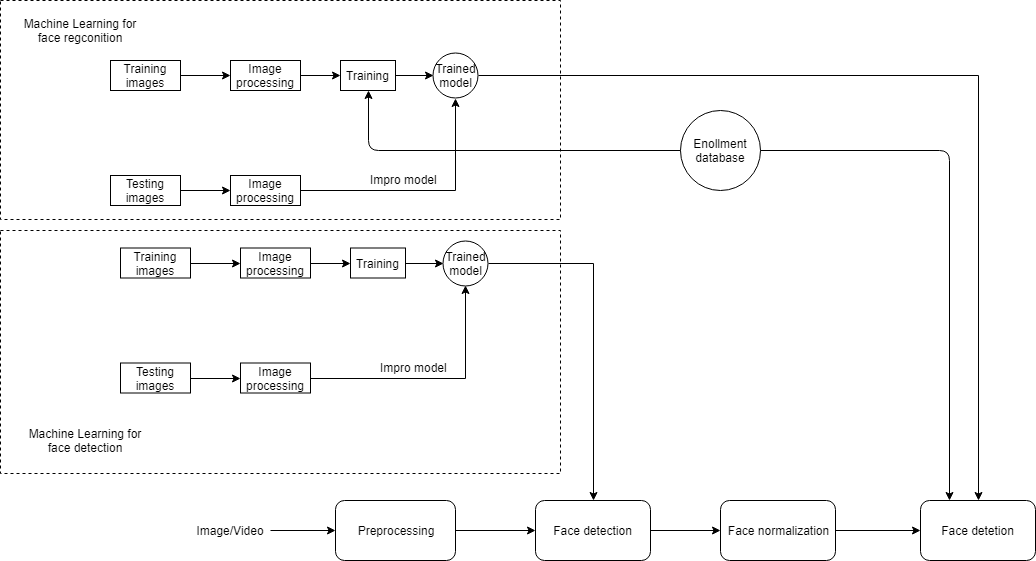
\includegraphics[width=\textwidth]{../images/fig/hinh4.png}
\caption{Sơ đồ tổng quát của bộ nhận diện khuôn mặt}../images/fig/hinh4.png
\label{fig:hinh4}
\end{figure}
%
\section{Zedboard}
Bo mạch Zedboard là một nền tảng phần cứng được xây dựng trên chip XC7Z020 là một vi mạch thuộc dòng ZynQ-7000 của hãng Xilinx. Chip XC7Z020 tích hợp bên trong nó một hệ vi xử lý (tên tiếng Anh là Processing System, được viết tắt là PS) và khối logic khả trình (tên tiếng Anh là Programmable Logic, được viết tắt là PL). Trong đó, hệ vi xử lý được xây dựng với trung tâm là bộ vi xử lý Cortex-A9 lõi kép cùng hệ thống truyền thông dạng bus AXI của hãng ARM. Khối logic khả trình bao gồm các tài nguyên logic có khả năng tái cấu hình và các khối phần cứng chuyên dụng (như các khối DSP48E1, RAM block) tương đương với một vi mạch FPGA dòng Artix-7 của Xilinx.  Bên cạnh đó bo mạch Zedboard cũng có rất nhiều các ngoại vi và các giao diện ghép nối khác cho phép khách hàng có thể phát triển rất nhiều các ứng dụng thuộc các lĩnh vực khác nhau trên nó..\cite{zedboard}. Những thành phần chính của bo mạch Zedboard như chỉ ra trong hình \ref{fig:zedboard}
\begin{itemize}
\item Máy thu nhúng có kết nối 10G + hiệu suất cao 
\item Nền tảng nhúng, có thể tùy chỉnh, công suất thấp không cần PC 
\item Tuổi thọ cao
\item Nền tảng lập trình hiệu quả cao : o Xử lý tầm nhìn hoàn hảo trong xử lý nối tiếp hiệu suất PLoHigh của thiết bị Zynq lên đến 1 GHz trong PS của thiết bị Zynq
\end{itemize}
Đặc điểm mà chúng ta cần sử dụng ở zedboard với bộ công cụ hỗ trợ tự Zynq, ta có thể sử dụng phần mềm Vivado để thực hiện lập trình C thay vì sử dụng verilog 
\begin{figure}[H]
\centering
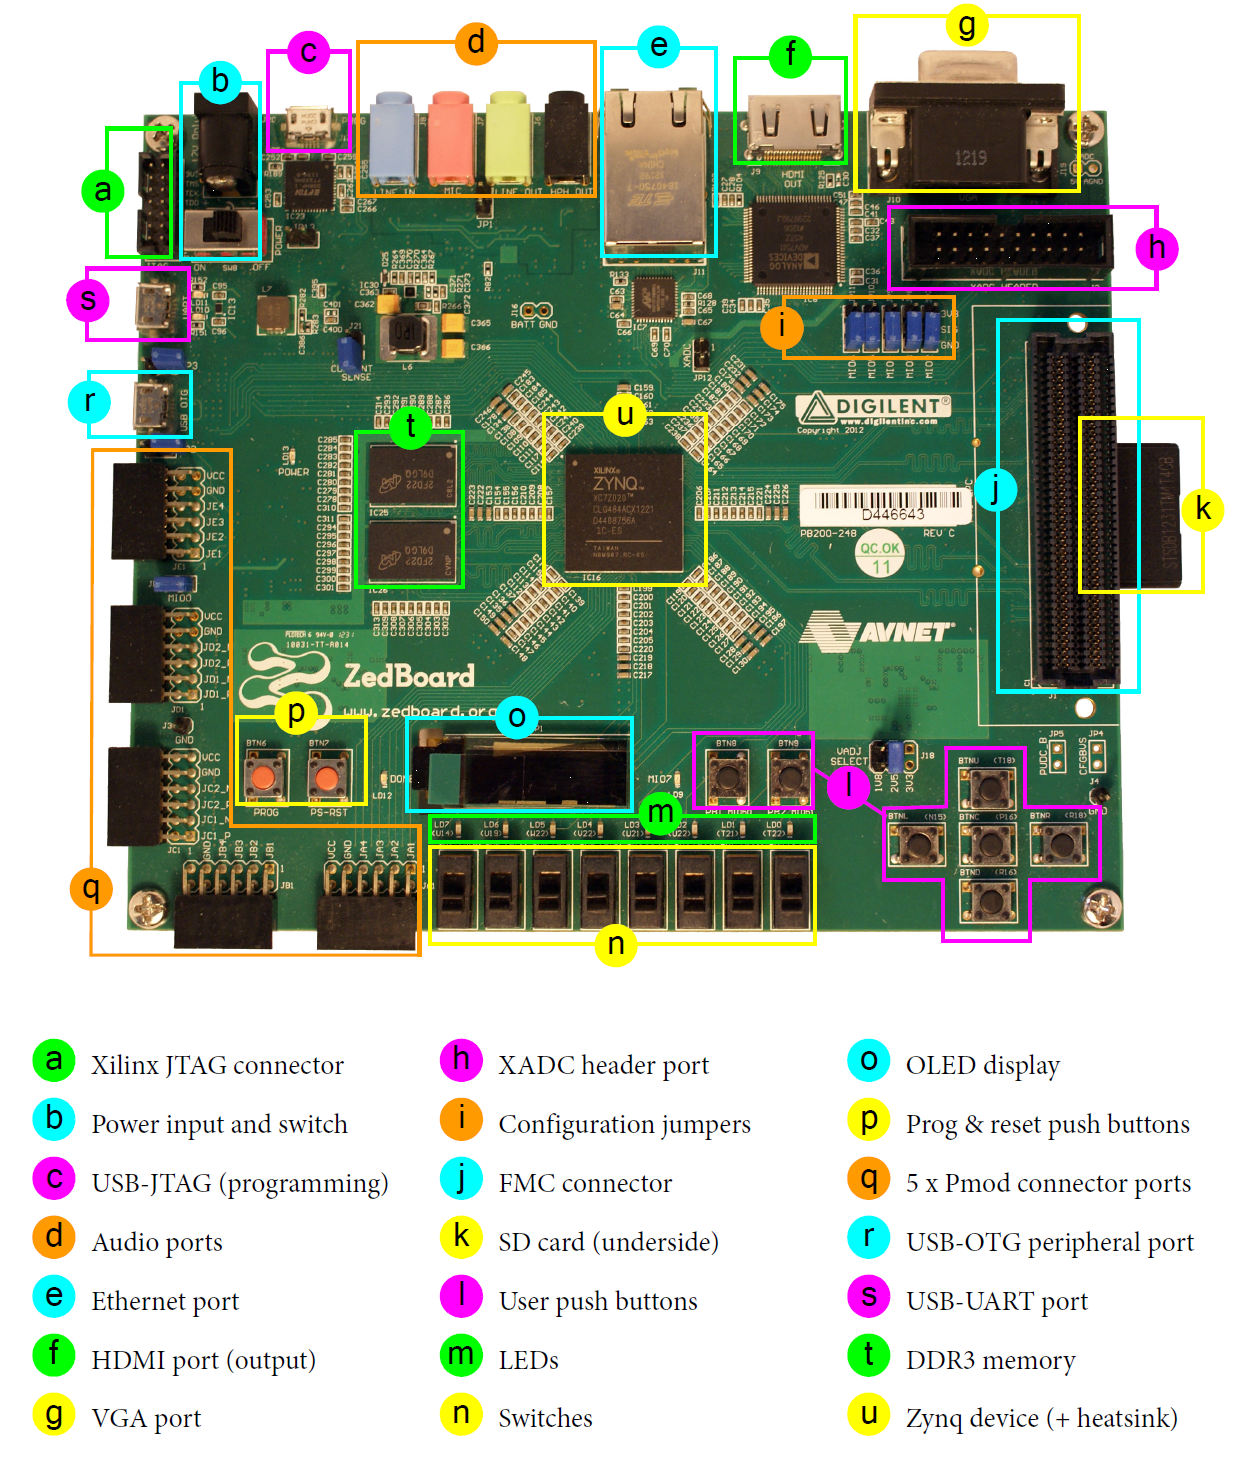
\includegraphics[width=.7\textwidth]{../images/fig/zedboard.png}
\caption{Bo mạch Zedobard}
\label{fig:zedboard}
\end{figure}
\section{Các giải thuật}
\subsection{Một số giải thuật Face Dectection}
Trước khi nhận diện được khuôn mặt, ta cần một giải thuật giúp cho việc phát hiện được khuôn mặt đã.
\subsubsection{Haar-cascade classifier}
Haar-cascade (Wilson \& Fernandez, 2006) là một phương pháp học máy phát minh bởi Viola và Jone (Viola \& Jones, 2001) dùng để phát hiện vật thể trong ảnh. Trong trường hợp này nó được dùng để phát hiện khuôn mặt. Tên của phương pháp này là từ ghép của 2 từ. Haar trong Haar-like features, là một bộ phân loại (classifier) yếu (tức chỉ nhỉnh hơn đoán ngẫu nhiên một ít). Một feature là một hình chữ nhật bị chia thành nhiều phần chữ nhật khác nhau, Mỗi hình sẽ có màu trắng hoặc đen. Hình \ref{fig:2.10} cho ta thấy các feature có thể có. Haar-cascade cần được train với rất nhiều hình positive (có mặt người) và negative (không có mặt người). Mục tiêu là để chiết xuất ra được một tập hợp các feature đại diện cho khuôn mặt. Giải thuật học máy này yêu cầu ảnh ở dạng đơn sắc. Cường độ của màu xám sẽ được dùng để xác định xem feature nào đang được đại diện. Những feature này có thể được tính toán bằng cách tính tổng các các pixel màu đen trong vùng trừ đi tổng của các pixel màu trắng.
%
\begin{figure}[H]
\centering
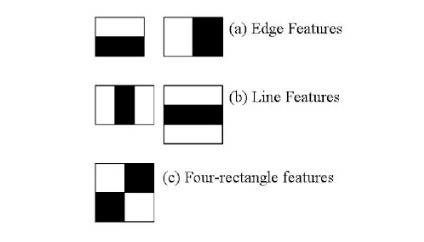
\includegraphics[width=.5\textwidth]{../images/fig/2-10.png}
\caption{Haar features dùng cho face detection}
\label{fig:2.10}
\end{figure}
%
\noindent
Như trong hình \ref{fig:2.11} Feature thứ nhất được chọn dựa trên việc tròng đen của mắt sẽ tối hơn tạo nên một feature đặt trưng và dễ nhận ra nhất. Feature thứ hai dựa trên việc phần 2 hốc mắt thường sẽ tối hơn phần sống mũi. Tất nhiên các feature ở cằm và mũi sẽ khó phát hiện hơn và cần nhiều công cụ hỗ trợ hơn.
%
\begin{figure}[H]
\centering
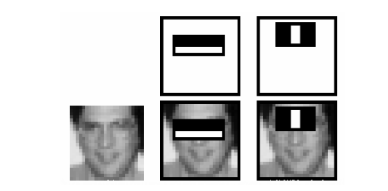
\includegraphics[width=.5\textwidth]{../images/fig/2-11.png}
\caption{Ví dụ 2 features chiết xuất được từ ảnh}
\label{fig:2.11}
\end{figure}
%
\noindent
Sự tổng hợp của các feature được chiết xuất ra từ ảnh sẽ được dùng để phát hiện khuôn mặt trong ảnh. Với một bức ảnh lạ thì sự tổng hợp này sẽ được xem xét để đưa ra quyết định xem nó có chứa khuôn mặt hay không. Các feature này sẽ chỉ nằm trong một vùng pixel định trước bởi một bộ scale. Một scale có thể là một vùng ô vuông 24x24 pixels. Mỗi feature trong tập hợp sẽ được thử lần lượt trong vùng. Nếu một trong các feature không xuất hiện trong vùng, việc xem xét sẽ dừng lại. Các feature còn lại sẽ không được thử vì khi đó thuật toán chỉ ra rằng không có khuôn mặt trong vùng này. Khi đó một vùng mới sẽ được thử, lặp lại như vậy. Phương pháp này thử tất cả các vùng pixels lần lượt như thác đổ (cascade).
\par\noindent
Phương pháp này hiệu quả trong việc xác định các bức ảnh không có khuôn mặt vì khi đó việc thử sẽ chỉ diễn ra đối với một vài feature trước khi nó xác nhận rằng không có khuôn mặt trong vùng đó và chuyển đến vùng kế. Ngược lại một khuôn mặt được xác định là tồn tại trong vùng đó nếu nó phù hợp với tất cả các feature trong khối tổng hợp feature trên nói trên. Hình \ref{fig:2.12} thể hiện một khối tổng hợp các feature nó dùng để "thử" các vùng. Tất cả các feature này được chiết xuất ra từ tập dữ liệu huấn liện để tìm ra các pattern đại diện cho khuôn mặt.
%
\begin{figure}[H]
\centering

\includegraphics[scale=.5]{../images/fig/2-12.png}
\caption{Ví dụ về tổng hợp của các feature (Arubas)}
\label{fig:2.12}
\end{figure}
%
\noindent
Quá trình thử sẽ thực hiện lần lượt các vùng cho đến vùng cuối cùng. Sau đó scale sẽ được tăng lên, và quá trình này sẽ được lặp lại. Điều này giúp cho giải thuật có thể nhận biết được khuôn mặt với nhiều kích thước khác nhau. Các vùng chỉ chênh nhau 1 vài pixel, nên việc phát hiện 1 khuôn mặt trong nhiều vùng sẽ xảy ra. Tất cả các khuôn mặt được cho là thuộc cùng 1 người sẽ được gom lại và xem như 1 người trong cuối quá trình. Bộ phân loại Haar-cascade chỉ cần train một lần nhưng lại có thể phát hiện khuôn mặt rất nhanh.
\subsubsection{Histogram of Oriented Gradients (HOG)}
HOG (Dalal \& Triggs, 2005) (Geitgey, 2016) là một phương pháp khác cũng dùng để phát hiện vật thể, cũng yêu cầu sử dụng ảnh đơn sắc. HOG so sánh mỗi pixel với lân cận của nó - thường là 8 pixels. Mục tiêu là để tìm ra xem ở hướng nào thì bức ảnh tối dần đi. Một mũi tên trắng sẽ được vẽ để biểu diễn hướng này. Như ta đã biết 0 biểu diễn màu đen, nên số càng nhỏ thì pixel đó càng tối. Điểm mạnh của phương pháp này là nó không nhạy cảm với cường độ sáng. Nếu bức ảnh đang tối đi, tất cả pixel sẽ tối đi. Mũi tên biểu diễn hướng tối đi sẽ không đổi dù bức ảnh có cường độ sáng hơn. Tuy nhiên điều này lại không đúng nếu nếu chỉ một phần của bức ảnh bị thay đổi độ sáng, chẳng hạn như bị đèn chiếu vào
\par\noindent
Bước này cho chúng ta hình dạng mà ta phân tích được từ các mũi tên, tuy nhiên nó lại có quá nhiều. Mục tiêu là phát hiện ra khuôn mặt trong khi quá nhiều chi tiết thừa chỉ để nhận biết một khuôn mặt. Vì thế, chỉ có những mũi tên chỉ hướng quan trọng được giữ lại. Bước tiếp theo ta cần chia bức ảnh thành các khối 16x16 pixels - gọi là square. Đếm xem có bao nhiêu lần mỗi hướng được phát hiện trước đó, và chỉ có một mũi tên được vẽ trong 1 square với hướng được phát hiện nhiều nhất. Thao tác này được thực hiện với tất cả square trong hình. Và kết quả sẽ cho ta một biểu diễn tổng quát của khuôn mặt. Tất cả các bước sẽ được thực hiện với số lượng lớn các mặt trước có sẵn để xác định pattern tốt nhất cho việc phát hiện khuôn mặt. Hình \ref{fig:2.13} biểu thị một khuôn mặt trung bình đã được train với 3000 bức ảnh sử dụng thư viện dlib.
%
\begin{figure}[H]
\centering
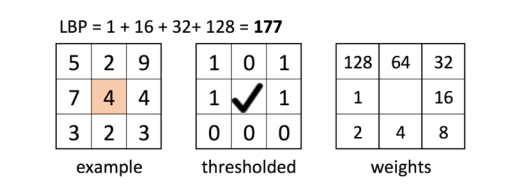
\includegraphics[width=.5\textwidth]{../images/fig/2-14.png}
\caption{Hình ảnh trực quan HOG detector tạo ra từ thư viện dblib}
\label{fig:2.13}
\end{figure}
%
\subsection{Một số giải thuật Face Regconition}
Có rất nhiều cách tiếp cận cũng như phương pháp cho việc nhận diện khuôn mặt. Giải thuật có thể dùng thống kê, cố tìm một pattern đại diện cho một người cụ thể hoặc dùng mạng nơ-ron tích chập. Các cách tiếp cận này có thể được tìm thấy trong các giải thuật được trình bày dưới đây.
\subsubsection{Eigenfaces}
Eigenfaces (Turk \& Pentland\cite{eigenface1}), (Morizet, Ea, Rossant, Amiel, \& Amara\cite{eigenface2}) là phương pháp nhận diện khuôn mặt dựa trên cách tiếp cận bằng thống kê. Mục tiêu của phương pháp này là trích xuất các thành phần đặc trưng có thể dùng để phân biệt khuôn mặt. Eigenfaces sử dụng cách tiếp cận toàn diện - dùng cả mặt, mỗi tập đại diện cho một người và không tính toán độ sai biệt giữa 2 bức ảnh trong 2 tập khác nha - nghĩa là quyết định cuối cùng phụ thuộc hoàn toàn vào giá trị trung bình của bức ảnh. Các bức ảnh đầu vào cần phải trải qua bước tiền xử lí để chuyển thành ảnh trắng đen. Mỗi pixel sẽ chỉ đại diện cho một chiều, nghĩa là bức ảnh trắng đen $96\times 96 =9216$ chiều. Eigenfaces được xây dựng dựa trên Principal Component Analysis (PCA) (Turk Pentland, 1991) (Morizet \& al., 2006) để giảm số chiều của dữ liệu mà vẫn giữ được những thông tin quan trọng. Quá trình train của Eigenfaces là để tính toán các eigenvectors và các giá trị eigenvalues tương ứng với ma trận hiệp phương sai của tập train.
\par\noindent
Ở bước test, khoảng cách Euclid hoặc Mahalanobis sẽ được dùng để tính toán độ sai biệt của bức ảnh đầu vào và tất cả ảnh, bức ảnh nào có giá trị này nhỏ nhất sẽ được chọn là kết quả dự đoán. 
\subsubsection{Fisherfaces}
Fisherfaces (Jaiswal \& al., 2011) (Morizet \& al., 2006) (Belhumeur, Hespanha, \& Kriegman \cite{fisherface1}) cũng áp dụng cách tiếp cận toàn diện như Eigenfaces, đó là sử dụng toàn bộ khuôn mặt, điểm khác biệt lớn nhất là Fisherfaces tính toán độ sai biệt giữa 2 tập khác nhau (2 người). Vì thế ngoài PCA, Fisherfaces còn dùng đến Linear Discriminant Analysis (Jaiswal \& al., 2011) (Morizet \& al., 2006) (Belhumeur \& al., 1997) để tính toán sự sai biệt giữa 2 bức ảnh trong 2 tập khác nhau - mục đích là để tối thiểu sai biệt giữa các bức ảnh của cùng một người và tăng độ sai biệt giữa 2 người khác nhau.
\par\noindent
Ở bước test, bức ảnh đầu vào sẽ được tính khoảng cách với tất cả ảnh trong cùng một tập và tất cả tập, tập nào bức ảnh thể hiện độ sai biệt thấp nhất sẽ là giá trị dự đoán.
\subsubsection{Local Binary Patterns Histograms (LBPH)}
Thuật toán này đòi hỏi hình ảnh đơn sắc để xử lý việc huấn luyện. Ngược lại với thuật toán trước, đây không phải là một cách tiếp cận toàn diện. Mục tiêu của LBPH (Ahonen, Hadid, \& Pietik \cite{local1}) (Mäenpää, Pietikäinen, \& Ojala \cite{local2}) (Di Huang \textit{et al.} \cite{local3}) là hoạt động theo các khối 3x3 pixel. Các pixel ở trung tâm được so sánh với pixel láng giềng. Với mỗi pixel láng giềng có giá trị nhỏ hơn pixel ở trung tâm thì giá trị 0 sẽ được thêm vào ma trận threshold ở vị trí tương ứng (hình \ref{fig:lbph1}, ngược lại thì là 1. Khi quá trình so sánh đã hoàn thành, mỗi pixel sẽ được nhân với trọng số tương ứng. Ma trận trọng số có giá trị từ $2^0 \rightarrow 2^7$ theo hình tròn và sẽ giữ nguyên giá trị đó ở tất cả bước so sánh. Sau đó tổng giá trị của 2 ma trận này sẽ là giá trị của pixel ở giữa hình. 
\begin{figure}[H]
\centering
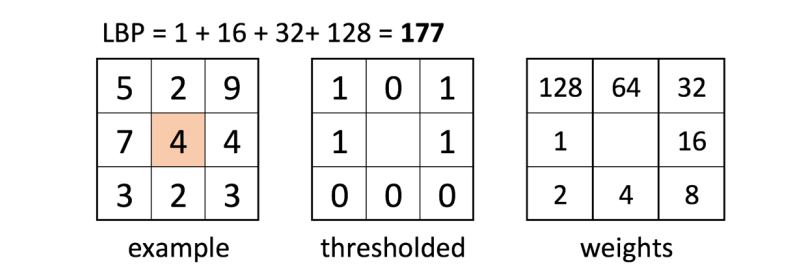
\includegraphics[scale=.5]{../images/fig/lbph1.png}
\caption{Các ma trận dùng trong giải thuật LBPH}
\label{fig:lbph1}
\end{figure}
Khi quá trình này đã được hoàn thành cho từng phần của bức ảnh, bức ảnh được chia thành một số vùng nhất định. Sau đó, một biểu đồ được trích xuất từ mỗi vùng và tất cả các biểu đồ được nối với nhau.
\par\noindent 
Ở bước test, quá trình tương tự được thực hiện và biểu đồ cuối cùng được so sánh với từng biểu đồ của bước train. Biểu đồ nào gần giống nhất là kết quả dự đoán của giải thuật. Đối với HOG detector, thuật toán này không nhạy cảm với sự thay đổi độ sáng.

%
\begin{figure}[H]
\centering
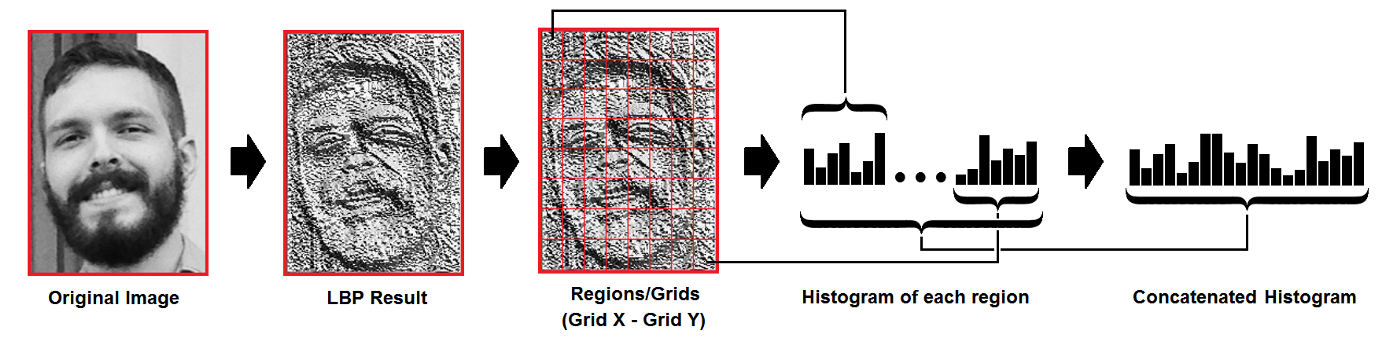
\includegraphics[width=.75\textwidth]{../images/fig/lbph2.png}
\caption{Quy trình của giải thuật LBPH}
\label{fig:lbph2}
\end{figure}
%

\subsubsection{Convolutional neural network (CNN)}
Ra đời dựa trên \cite{oldcnn1, oldcnn2}, CNN hoạt động theo phương thức nhận input và biến đổi input thông qua các layer, tuy nhiên điểm khác biệt nằm ở cấu trúc của input và cấu trúc bên trong 1 layer. 
\par\noindent
Lấy cảm hứng từ xử lý ảnh nên input của CNN có dạng như một bức ảnh chứ không có dạng vector như ANN, cụ thể một bức ảnh sau khi số hoá có dạng width x height x depth (width: số lượng điểm ảnh trên chiều rộng, height: số lượng điểm ảnh trên chiều cao, depth: số lượng kênh chẳng hạn như RGB có 3 kênh đại diện cho mức độ của 3 màu Đỏ, Lục, Lam) nên input của CNN là 1 tensor 3 chiều.
\par\noindent
\begin{itemize}
\item[-] Scalar : số vô hướng hay các số trong hệ thập phân ta vẫn sử dụng (5, 10, 7.2,…)
\item[-] Vector : là một tập các số vô hướng. Số lượng số vô hướng là số chiều của vector 
\item[-] Matrix : là một bảng hình chữ nhật được chia ô như bàn cờ, với mỗi ô là một số vô hướng. Một cách định nghĩa khác là matrix $mxn$ là tập hợp m vector n chiều.
\item[-] Tensor : phát triển lên từ các khái niệm trên ta có định nghĩa tensor, mỗi tensor n chiều là 1 tập các tensor n-1 chiều có cùng kích thước. Chẳng hạn Scalar là tensor 0D (0 Dimention – 0 chiều), Vector là tensor 1D, Matrix là tensor 2D… "
\end{itemize}
\noindent
Một CNN cơ bản gồm có các lớp như convolutional layer để filter các feature đặc trưng, max pooling layer đi sau để giảm chiều của dữ liệu và một hàm kích hoạt ReLu hay Sigmoid để cho ra kết quả về trọng số. Sau đó tất cả ma trận sẽ được làm phẳng để đi qua lớp cuối là Fully-connected layer bao gồm các layer liên kết đầy đủ với nhau bên trong, kết quả cuối cùng sẽ là nơi có giá trị dự đoán cao nhất (xem hình \ref{fig:cnn})
%
\begin{figure}[H]
\centering
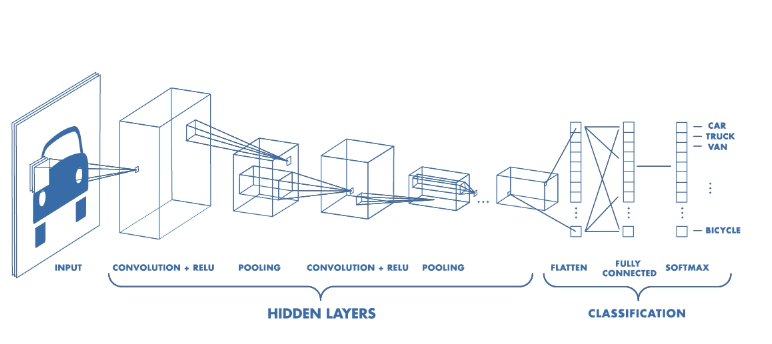
\includegraphics[width=.75\textwidth]{../images/fig/cnn.png}
\caption{Sơ đồ tổng quát của một CNN}
\label{fig:cnn}
\end{figure}
%
Đặc điểm của CNN là nó có thể nhận diện khuôn mặt mà không bị phụ thuộc vào một vị trí cố định của khuôn mặt trên bức ảnh, không những thế việc nó có thể tự tách các feature đặc trưng thông qua các bộ lọc đã là một lợi thế tuyệt vời khi không cần phải định nghĩa trước cho nó thế nào là một khuôn mặt hay các feature cụ thể. CNN đang là một xu hướng được áp dụng trong tất cả bài toán của Machine Learning, và nhận diện khuôn mặt không phải là một ngoại lệ
\subsubsection{OpenFace}
OpenFace (Amos, Ludwiczuk, \& Satyanarayanan, 2016) là một thư viện nhận dạng khuôn mặt. Nó dựa trên các hệ thống Google Face FaceNet (Schroff \& al.). OpenFace đang sử dụng DNN để thực hiện nhận dạng khuôn mặt. Nó sử dụng một phiên bản sửa đổi của mạng nn4 từ FaceNet. OpenFace được đào tạo với 500.000 hình ảnh. Như trong hình \ref{fig:openface}, cấu trúc được chia thành hai phần. 
%
\begin{figure}[H]
\centering
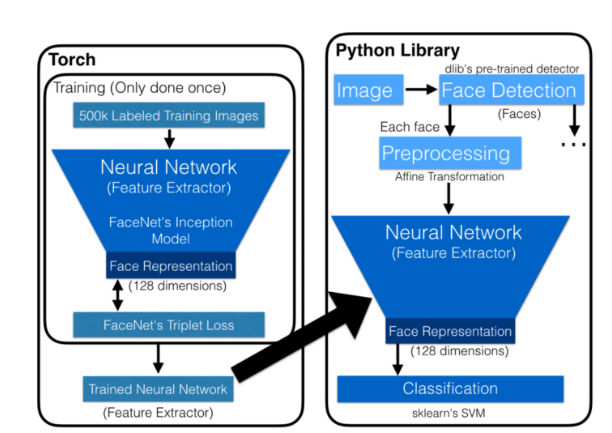
\includegraphics[scale=.5]{../images/fig/2-23.png}
\caption{Cấu trúc của dự án OpenFace (Amos \& al., 2016)}
\label{fig:openface}
\end{figure}
%
Ở bên trái, DNN được sử dụng để trích xuất các tính năng, kết quả có thể được sử dụng trực tiếp trong phần thứ hai của cấu trúc. Phần thứ hai của cấu trúc đòi hỏi một số hình ảnh cho mỗi đối tượng. Các khuôn mặt được phát hiện và trích xuất từ các bức ảnh bằng máy dò tiền đạo tạo của dlib sử dụng HOG. Sau đó, các gương mặt trải qua giai đoạn tiền xử lý và cuối cùng được sử dụng trong mạng nơ ron tích chập. CNN sử dụng các tính năng được trích xuất trong mạng nơ ron sâu từ phần bên trái của cấu trúc làm bộ lọc. Trong giai đoạn huấn luyện, CNN được điều chỉnh theo các lớp khác nhau. Để dự đoán một người không xác định, một hình ảnh được truyền qua phần bên phải của cấu trúc và lớp đại diện cho người đó sẽ được đưa ra làm đầu ra.
%-------------------------------------------------------------------------------------------

\section{Các công trình liên quan}
\subsection{Quốc tế}
\subsubsection*{Bài báo về "Hardware architecture design of face recognition system based on FPGA" \cite{ctquocte1}}
Thiết kế, hiện thực và kiểm nghiệm sử dụng chip cyclone III Field Programmable Gate Array (FPGA). board phát triển Altera DE0 được dùng để debug. giải thuật là PCA và FFT. Lợi thế của việc phát triển hệ thống này trên FPGA là khả năng cập nhật hoặc sửa lỗi bằng cách lập trình lại FPGA. Mục đích của hệ thống gồm kiểm soát ra vào, xây dựng CSDL khuôn mặt, nhận dạng, tương tác với con người... Dữ liệu ảnh có sự đa dạng về kiểu như độ sáng, mỉm cười. Kết quả thu được giải thuật PCA cho kết quả tốt hơn với những biến động trên, FFT có thể nhận diện được mặt người nhưng nếu cười hoặc độ sáng quá cao sẽ cho kết quả không tốt nhưng bù lại nhanh hơn trên phần cứng phù hợp để xử lý dữ liệu thời gian thực hơn PCA.
\subsubsection*{Bài báo về "Implementation of a face detection algorithm on a reconfigurable platform" \cite{ctquocte2}}
Áp dụng phương pháp linear spatial và temporal filter theo thời gian thực với video frame thu từ camera OV7670 sử dụng board Zynq Evaluation and Development board chạy trên chip Xilinx XC7Z020. Hệ thống được hiện thực hoàn toàn trên phần cứng, có thể phát hiện và track mặt người theo thời gian thực. Thực nghiệm cho thấy hệ thống có thể hoạt động với những nền sáng khác nhau không gây ảnh hưởng nhiều tới kết quả cuối cùng. Và hệ thống có thể loại bỏ nhiễu khung nền  tương đối tốt. tuy nhiên do sử dụng màu da người để nhận diện có thể nhận lầm những vật thể có màu giống da người thành mặt người, dù đã được erode bớt bởi 2 giải thuật linear spatial và temporal filter . Và một trong những vấn đề với hệ thống là vì tài nguyên hệ thống có giới hạn nên chỉ có thể tạo 1 số lượng detector nhất định nên không thể track được toàn bộ nếu có nhiều người và ngoài ra còn một số khó khăn vì ảnh thu được từ camera bị mờ và màu ảnh bị biến dạng dẫn tới kết quả không chính xác.
\subsection{Trong nước}
\subsubsection*{Thiết kế SOPC cho ứng dụng nhận dạng mặt người dùng thuật toán WMPCA \cite{cttrongnuoc}}
Phần cứng gia tốc cho kỹ thuật lượng tử hóa vevctor (Vector Quantization) đã được phát triển thành một thành phần nhúng (system on a programable chip - SoPC)  trong các ứng dụng nén và nhận dạng ảnh thời gian thực. Ngày nay kỹ thuật FPGA kết hợp với công cụ SoPC cho thấy hiệu quả cao trong việc thiết kế các ứng dụng phần cứng gia tốc. Trong bài nghiên cứu này sẽ tìm hiểu hiệu quả của việc ứng dụng kiến trúc song song dựa trên thuật toán WMPCA và kiến trúc SoPC để nhận dạng mặt người online. Giải thuật WMPCA này nhằm loai bỏ những vùng ảnh chứa ít thông tin nhận dạng và tập trung vào những vùng ảnh quan trọng. Hệ thống được test trên  board  DSP Development Kit, stratix II professional Edition FPGA FP2S180. Thực nghiệm cho thấy hiệu quả phần cứng luôn nhanh hơn phần mềm, phần mềm thực hiện 7.5ms trên laptop intel core2, trong khi phần cứng đạt 1.6 ms trên FPGA ở 100mhz. Tài nguyên tiêu tốn cho một tập dữ liệu 100 trường hợp cho 10 đối tượng là 23\% tài nguyên chip FPGA, nên hoàn toàn có thể mở rộng áp dụng thực tế vào công nghiệp cũng như nghiên cứu. Đặc tính hệ thống phù hợp cho ứng dụng thời gian thực. Cho kết quả giữa phần cứng và phần mềm gần như trùng khớp nhau

\chapter{Thiết kế}
\section{Phân tích vấn đề}
Để thực hiện bài toán nhận diện khuôn mặt, hiện nay có rất nhiều giải thuật hỗ trợ cho vấn đề này, đơn cử như Python và C++ với bộ thư viện hỗ trợ đồ sộ, như OpenCV. Như vậy, để có thể thực hiện giải thuật của bài toán nhận diện, ta chỉ cần một thiết bị phần cứng hỗ trợ sử dụng một trong 2 loại ngôn ngữ này. 
\par\noindent 
Với sự phát triển cũng như nhu cầu của bài toán nhận diện mặt, các bộ data được tạo ra phục vụ cho nhu cầu thử nghiệm hiệu quả của giải thuật là cực kì khổng lồ, có thể kể đến các bộ data phổ biến \cite{dataset} như:
\begin{itemize}
\item \href{http://www.nist.gov/itl/iad/ig/colorferet.cfm}{The Color FERET Database, USA}: 1199 người, 14,126 ảnh, có màu, điều kiện phòng chụp .
\item \href{http://www.scface.org/}{SCface - Surveillance Cameras Face Database}: 130 người, 4160 ảnh, có màu, điều kiện camera thông dụng.
\item \href{http://www.multipie.org/}{Multi-PIE}: 337 người, 750.000 ảnh, 15 góc chụp và 19 điều kiện chiếu sáng.
\item \href{http://cbcl.mit.edu/software-datasets/heisele/facerecognition-database.html}{MIT-CBCL Face Recognition Database}: 10 người, 2 tập train, tĩnh và 3, chụp mặt, nghiêng và nghiêng một nửa.D
\item ...
\end{itemize}
Với việc giới hạn của đề tài là không quá lớn, nên ta cần lựa chọn hợp lí bộ data và kì vọng của giải thuật hợp lí
\par\noindent
Vì ứng dụng của đề tài muốn có thể áp dụng lên board, điều này là hợp lí vì với sức mạnh tính toán của fpga, ta có thể tăng tốc độ của giải thuật lên rất cao, tuy nhiên việc hiện thực ngôn ngữ C trở thành verilog có thể được hỗ trợ bởi phần mềm vivado HLS, nhưng việc sử dụng bộ thư viện đồ sộ của OpenCV cho việc này là một trở ngại lớn. Vậy nên ta sẽ lợi dụng Processing System để điều khiển Programmable logic trên board. Điều này lại gây ra một vấn đề khác khi hệ điều hành có sẵn trên board không cung cấp compiler, công cụ debug cũng như thư viện cần thiết để thực hiện.
\par\noindent
Cuối cùng là giải thuật để nhận diện khuôn mặt, với số lượng giải thuật nhiều như hiện tại, đề tài sẽ sử dụng một giải thuật đã có sẵn mà mang lại hiệu quả tốt chứ không tập trung phát triển một giải thuật mới.

\section{Lựa chọn giải pháp}
Với các vấn đề đã phân tích ở trên, nhóm quyết định lựa chọn giải pháp sử dụng ngôn ngữ C++ để thực hiện nhận diện khuôn mặt. Theo \cite{sosanh}, cũng như các kết quả  từ việc kiểm thử trong thực tế trên bộ dữ liệu của \href{https://cswww.essex.ac.uk/mv/allfaces/faces94.html}{face94}, độ phức tạp của việc hiện thực, Haar-cascade classifier kết hợp cùng với Local Binary Pattern Histogram(LBPH) đem lại kết quả lí tưởng nhất cho đề tài này. Bộ dữ liệu SCface với điều kiện camera cũng là lựa chọn hợp lí cho việc nhận diện thông qua camera trong phòng thí nghiệm chủ yếu là các sinh viên - các kết quả của bài báo cáo cũng như phần hiện thực sẽ được thực hiện dựa trên giải thuật LBPH, dùng model Face Detection sử dụng Haar Cascadesvà bộ dữ liệu faces94 kết hợp với bộ dữ liệu về các thành viên của nhóm.
\par\noindent
Việc hiện thực code lên board sẽ được sử dụng bằng SDK Xilinx, như đã đề cập ở trên về hệ điều hành. Có rất nhiều giải pháp cho việc lựa chọn hệ điều hành, nhưng nhóm sẽ sử dụng hệ điều hành Petalinux, được hỗ trợ bởi Xilinx\cite{peta}, và có sẵn Zedboard Standalone Board Support Package (BSP), có nguồn tài liệu phong phú cũng như việc build hệ điều hành cũng không quá phức tạp.
\section{Thiết kế}
Công cụ:
\begin{itemize}
\item ZedBoard Zynq-7000 ARM/FPGA SoC Development Board
\item Xilinx SDK 
\item Petalinux 
\item Open CV 3.3.0 
\item FFMPEG 2.18.5
\end{itemize}
Kết hợp từ tập dữ liệu face94 và hình ảnh tự tạo của các thành viên, sử dụng chương trình cắt hình ảnh đúng với kích thước các hình ảnh của face94 vì giải thuật yêu cầu các ảnh đầu vào phải có cùng kích thước (hình \ref{fig:thietke2})
%
\begin{figure}[H]
\centering
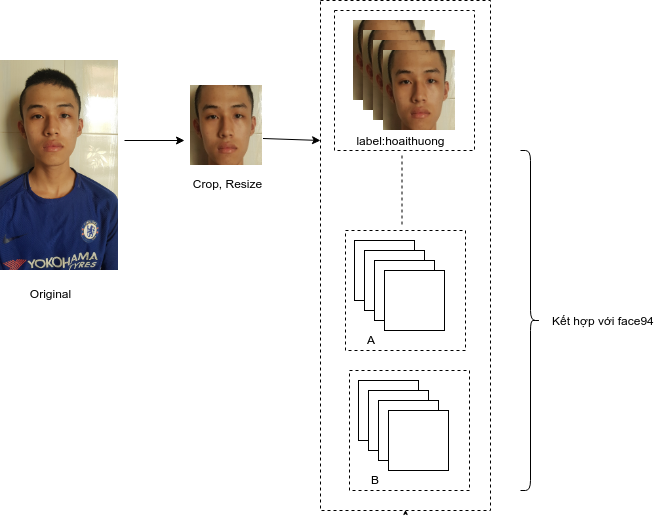
\includegraphics[scale=.5]{../images/fig/thietke2.png}
\caption{Chuẩn bị tập dữ liệu đầu vào}
\label{fig:thietke2}
\end{figure}
%
oindent
Chia tập train, test và validation theo tỉ lệ 60/20/20, lưu lại vào file csv chứa địa chỉ đến hình ảnh và nhãn của mỗi ảnh (hình \ref{csv})
%
\begin{figure}[H]
\centering
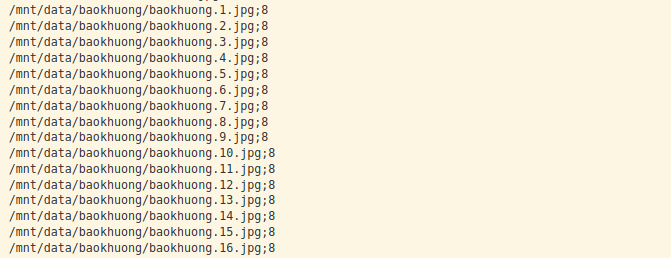
\includegraphics[scale=.5]{../images/fig/csv.png}
\caption{Cấu trúc các sample trên file csv}
\label{csv}
\end{figure}
%
Quá trình xử lí hình ảnh của Local Binary Patterns Histograms được thể hiện như hình \ref{fig:thietke3}
%
\begin{figure}[H]
\centering
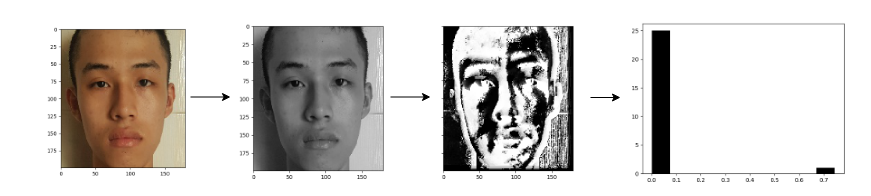
\includegraphics[scale=.5]{../images/fig/thietke3.png}
\caption{Quy trình của LPBH}
\label{fig:thietke3}
\end{figure}
%
Đoạn code sau minh hoạ việc hiện thực giải thuật LBPH\\
\lstinputlisting[language=cpp, title={LBPH sử dụng neighbor và radious để tính toán giá trị}]{../code/elph.cpp} 
\lstinputlisting[language=cpp, title={Chuyển ma trận thành dạng histogram}]{../code/histogram.cpp}
\lstinputlisting[language=cpp, title={Quá trình train, gắn các histogram vào nhau}]{../code/train.cpp} 
\lstinputlisting[language=cpp, title={Quá trình dự đoán dựa trên histogram có độ sai biệt thấp nhất}]{../code/predict.cpp}  
\subsubsection*{Kết hợp toàn bộ, ta có sơ đồ tổng quát của hệ thống được minh hoạ như hình \ref{fig:thietke1}}
%
\begin{figure}[H]
\centering
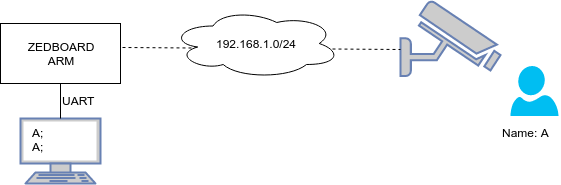
\includegraphics[scale=.5]{../images/fig/thietke1.png}
\caption{Sơ đồ tổng quát của cả hệ thống}
\label{fig:thietke1}
\end{figure}
%
\section{Hiện thực}
\subsection{Hiện thực với chương trình C++ trên thiết bị khác}
Việc hiện thực trước trên thiết bị hỗ trợ nhiều hơn giúp ta sửa các lỗi dễ dàng hơn tiết kiệm thời gian làm việc trên board. Sau khi thực hiện bước này, những thứ ta đã có bao gồm:
\begin{itemize}
\item Tập dữ liệu train, validation, test (bao gồm khuôn mặt cá nhân muốn nhận diện)
\item Source code C++ của chương trình
\end{itemize}
%
\begin{figure}[H]
\label{baohan}
\centering
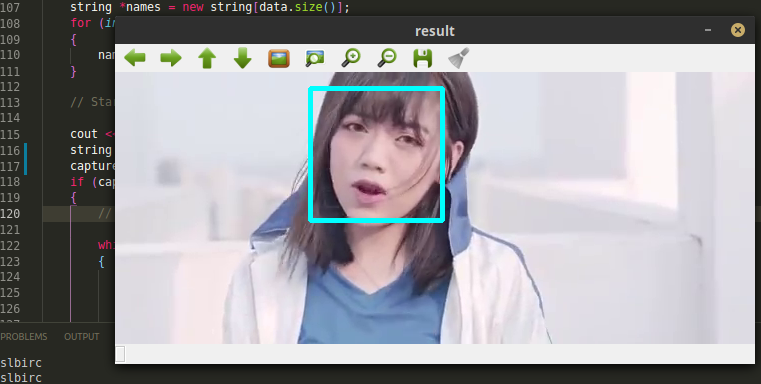
\includegraphics[scale=.5]{../images/fig/baohan.png}
\caption{Ví dụ hiện thực trên Ubuntu}
\end{figure}
%
\subsection{Hiện thực lên board}
Chuẩn bị:
\begin{enumerate}
\item Bản build của hệ điều hành petalinux đã cài đặt tcf-agent, opencv, gcc-run-time-xoject (xem phụ lục  \ref{section:buildpetalinux})
\item Cài đặt Xilinx SDK
\end{enumerate}
Hiện thực:
\begin{enumerate}
\item Kết nối với Zedboard thông qua UART
\item Boot Petalinux đã build ở trên, ở đây nhóm boot thông qua SD card (xem phụ lục \ref{section:sdcard})
\item Điều chỉnh card mạng của zedboard kết nối với host chứa Xilinx SDK thông qua ifconfig 
\item Mở Xilinx SDK, tạo application project, sử dụng source code đã hiện thực ở trên, build project và chọn Run project lên board thông qua Linux-agent (xem phụ lục \ref{sdkguide})
\item Cross-compiler FFMPEG để thư viện OpenCV trên Petalinux có thể sử dụng được và đọc giá trị từ camera (xem phụ lục \ref{ffmpeg})
\item Sử dụng một IP camera để ghi nhận hình ảnh, chạy chương trình để kết nối với Camera đó và xem kết quả

\end{enumerate}
\chapter{Kết quả và đánh giá}
\section{Kết quả}

Kết quả của chương trình khi sử dụng IP camera nhận diện trực tiếp (hình \ref{fig:ketqua1}), terminal của zedboard in ra kết quả mà nó dự đoán. 
%
\begin{figure}[H]
\centering
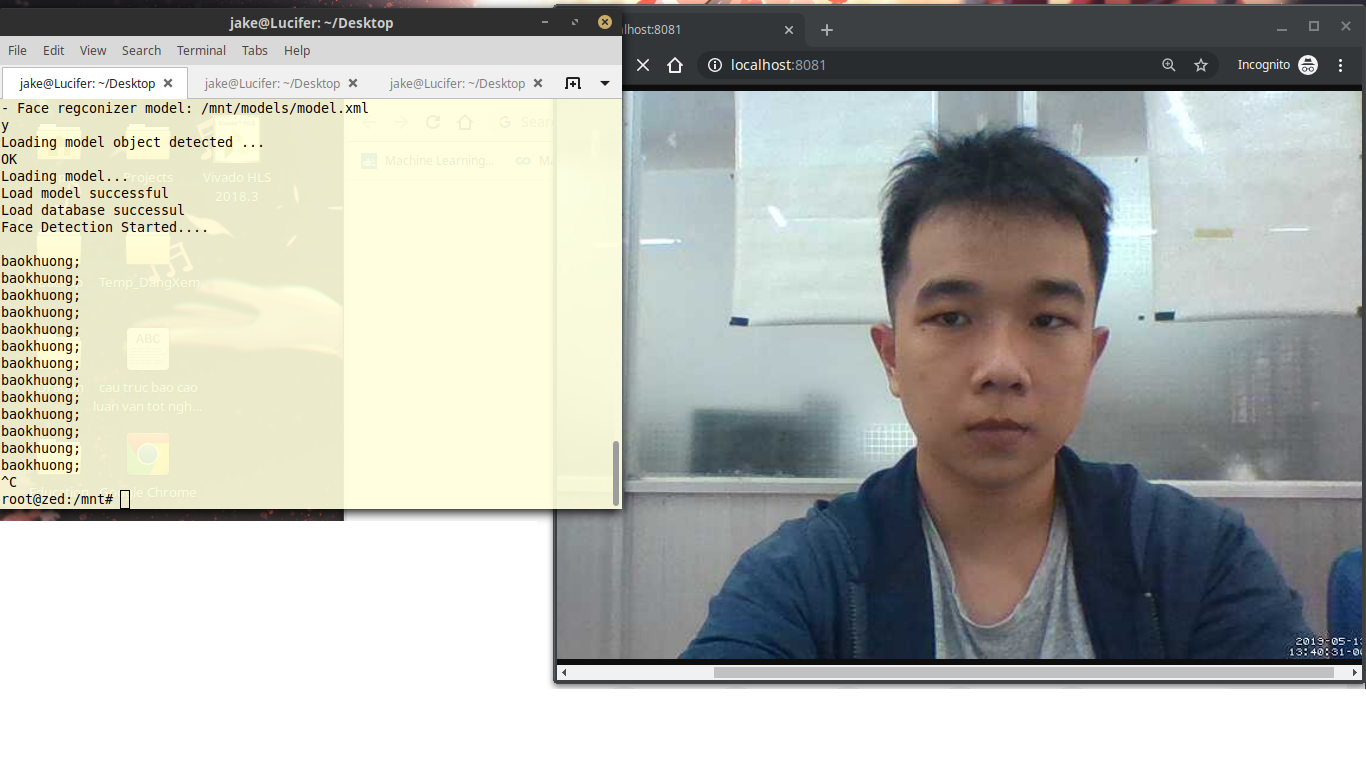
\includegraphics[width=.8\textwidth]{../images/fig/ketqua1.png}
\caption{Kết quả khi hiện thực với IP camera laptop}
\label{fig:ketqua1}
\end{figure}
%
\par \noindent 
Kết quả khi xuất ra video (hình \ref{fig:ketqua2}), ở đây hệ thống sẽ ghi lại các frame mà nó đọc được từ camera hoặc video, vẽ khung, ghi nhãn cho khuôn mặt nó nhận diện được và xuất ra video. 

\begin{figure}[H]
\centering
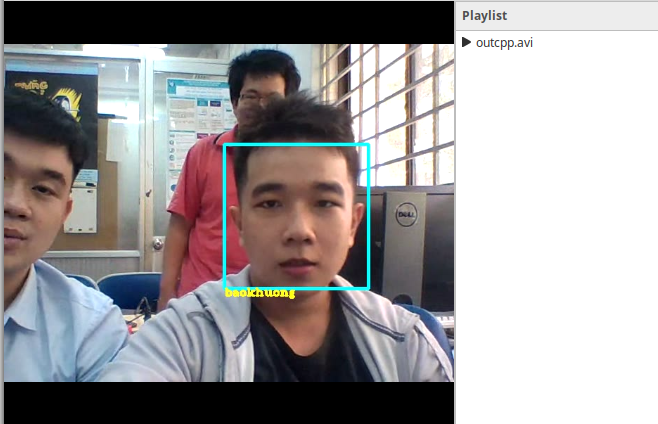
\includegraphics[width=.8\textwidth]{../images/fig/video1.png}
\caption{Một frame từ video được tạo ra với dữ liệu IP camera của zedboard}
\label{fig:ketqua2}
\end{figure}


\section{Đánh giá}
So với tốc độ xử lí ở các thiết bị hiện đại, tốc độ xử lí của zedboard là khá chậm, tuy nhiên độ chính xác của giải thuật thì vẫn chấp nhận được. Bảng \ref{table:sosanh} so sánh thời gian xử lí hết 1 video có 541 frame hình so với máy tính intel core i5.

\begin{table}[H]
\centering
\begin{tabular}{|l|l|l}
\cline{1-2}
CPU           				& Time (s)    				&  \\ \cline{1-2}
ARM Cortex-A9 		& $1208.885052$ 		&  \\ \cline{1-2}
Intel core i5 				& $78.751894$  			 &  \\ \cline{1-2}
\end{tabular}
\caption{So sánh thời gian xử lý 541 frame hình của 2 CPU}
\label{table:sosanh}
\end{table} 

Bảng \ref{table:sosanh2} cho thấy thời gian và độ chính xác của 3 giải thuật thực hiện trên ARM Cortex-A9 với bộ dữ liệu gồm 364 mẫu cho thử nghiệm về thời gian train, 1616 mẫu, 100 labels với 454 mẫu test cho độ chính xác
\begin{table}[H]
\centering
\begin{tabular}{|l|r|r|}
\hline
\multicolumn{1}{|c|}{Giải thuật} 	& \multicolumn{1}{c|}{Time (s)} 		& \multicolumn{1}{|c|}{Độ chính xác} \\ \hline
LBPH                            				& $12,611,357$                    			&  $0.997797$                                     \\ \hline
Eigenfaces                       			& $298,340,586$                   			&  $0.999998$                                             \\ \hline
Fisherfaces                     				& $241,654,857$                  			&  $0.995595$                                            \\ \hline
\end{tabular}
\caption{Thời gian và độ chính xác của 3 giải thuật thực hiện trên ARM}
\label{table:sosanh2}
\end{table}
Với kết quả như ở bảng \ref{table:sosanh2}, việc lựa chọn giải thuật LBPH là hợp lí cả về thời gian và độ chính xác, nhất là khi cân nhắc tốc độ xử lí của ARM, việc LBPH tiêu tốn thời gian ít hơn 2 giải thuật còn lại nhiều lần là một điểm cực kì sáng giá. Điều này cũng phản ánh đúng phần nào kết quả của khảo sát \cite{sosanh}
\chapter{Kết luận, thảo luận và khuyến nghị}
\section{Kết luận}
\subsection{Các mục tiêu đã đạt được}
\begin{itemize}
\item Nhận diện được người thông qua camera giám sát.
\item Sử dụng zedboard để thực hiện nhận diện.
\item Độ chính xác của chương trình nằm ở mức chấp nhận và có thể phát hiện người lạ.
\end{itemize}
oindent
\subsection{Các mục tiêu chưa đạt}
\begin{itemize}
\item Sử dụng FPGA để thực hiện việc tính toán trong quá trình training thay vì sử dụng ARM
\item Chưa thể dùng zedboard để khoanh vùng (boxing) khuôn mặt như khi thực hiện trên thiết bị khác. 
\end{itemize}
\subsection{Kết quả đạt được về chuyên môn}
\begin{itemize}
\item Nhóm đã có thêm sự hiểu biết về lập trình với zedboard, sử dụng được Vivado và Xilinx SDK 
\item Thử nghiệm các giải thuật nhận diện khuôn mặt khác nhau như Eigenfaces, Fisherfaces và LBPH, đồng thời tìm hiểu thêm được về neural network và các lý thuyết khác xung quanh machine learning.
\item Thực hành được thêm với zedboard, với hệ điều hành Linux, với các công cụ debug, sửa lỗi, ...
\end{itemize}

\section{Hướng phát triển}
Vì thời gian và nguồn lực có hạn, trong quá trình thực hiện đề tài, nhóm chỉ có thể thực hiện :
\begin{enumerate}
\item Làm quen với zedboard, Xilinx SDK
\item Build, Config và boot Petalinux có kết hợp OpenCV và FFMpeg cho ARM 
\item Viết chương trình nhận diện khuôn mặt sử dụng giải thuật Haar để xác định vật thể và LBPH để train model nhận diện
\item Liên kết chương trình với IP camera thông qua cổng ethernet trên zedboard
\end{enumerate} 
Với nền tảng đó, chương trình về sau có thể phát triển thêm bằng cách:
\begin{enumerate}
\item Sử dụng FPGA cho việc huấn luyện, thậm chí là predict, vì Petalinux hỗ trợ cho PS của zedboard giao tiếp được với PL
\item Chuyển luồng dữ liệu từ camera hoặc video sang cổng HDMI hoặc VGA để hiện lên màn hình, đồng thời đóng khung và hiện luôn giá trị dự đoán lên màn hình đó.
\item Sử dụng các giải thuật hiệu quả hơn LBPH và model nhận diện vật thể hiệu quả hơn Haar
\end{enumerate}

\cleardoublepage
\chapter{Phụ lục}
%\renewcommand\thesubsection{\Alph{section}}

\section{Lịch và kế hoạch làm việc}

\begin{table}[H]
\resizebox{\textwidth}{!}{%
\begin{tabular}{|c|c|l|l|}
\hline
Tuần & Giai đoạn & \multicolumn{1}{c|}{Mục tiêu} & \multicolumn{1}{c|}{Yêu cầu} \\ \hline
7 & \multirow{4}{*}{\begin{tabular}[c]{@{}c@{}}1. Tìm hiểu yêu \\ cầu đề bài\end{tabular}} & \multirow{4}{*}{\begin{tabular}[c]{@{}l@{}}Tìm hiểu kiến thức nền tảng \\ và công trình liên quan\end{tabular}} & \multirow{4}{*}{\begin{tabular}[c]{@{}l@{}}- Tìm hiểu các cơ sở lý thuyết về nhận diện khuôn mặt\\ - Tìm hiểu về các project sử dụng trên zedboard\\ - Tìm hiểu cách sử dụng zedboard\\ - Đặt ra các tiêu chí và kì vọng của project\end{tabular}} \\ \cline{1-1}
8 &  &  &  \\ \cline{1-1}
9 &  &  &  \\ \cline{1-1}
10 &  &  &  \\ \hline
11 & \multirow{6}{*}{\begin{tabular}[c]{@{}c@{}}2. Thiết kế + mô phỏng \\ trên phần mềm\end{tabular}} & \multirow{2}{*}{Chọn ra phương án thiết kế} & \multirow{2}{*}{\begin{tabular}[c]{@{}l@{}}- Giải thích được tại sao lại lựa chọn phương \\ án thiết kế này + hiểu các lý thuyết liên quan\end{tabular}} \\ \cline{1-1}
12 &  &  &  \\ \cline{1-1} \cline{3-4} 
13 &  & \multirow{2}{*}{\begin{tabular}[c]{@{}l@{}}Thiết kế framework \\ (module cho việc training)\end{tabular}} & \multirow{2}{*}{\begin{tabular}[c]{@{}l@{}}- Chuẩn bị giải thuật\\ - Chuẩn bị tập train, test\end{tabular}} \\ \cline{1-1}
14 &  &  &  \\ \cline{1-1} \cline{3-4} 
15 &  & Hiện thực trên phần mềm & \begin{tabular}[c]{@{}l@{}}- Kết quả phải thoả các kì vọng đặt ra \\ để sau này có thể chạy lên board\end{tabular} \\ \cline{1-1} \cline{3-4} 
16 &  & \begin{tabular}[c]{@{}l@{}}Đánh giá, chỉnh sửa và tối \\ ưu giải thuật\end{tabular} & - Chạy so sánh với các giải thuật khác \\ \hline
17 & \multirow{5}{*}{\begin{tabular}[c]{@{}c@{}}3. Hiện thực trên \\ thiết bị\end{tabular}} & \multirow{3}{*}{Hiện thực, kiểm tra} & \multirow{3}{*}{\begin{tabular}[c]{@{}l@{}}- Giải thuật chạy cho kết quả giống như \\ khi thực hiện trên phần mềm\end{tabular}} \\ \cline{1-1}
18 &  &  &  \\ \cline{1-1}
19 &  &  &  \\ \cline{1-1} \cline{3-4} 
20 &  & Đánh giá kết quả & \begin{tabular}[c]{@{}l@{}}- Thu thập số liệu, đánh giá các\\ kết quả thu thập được\end{tabular} \\ \cline{1-1} \cline{3-4} 
21 &  & Báo cáo & - Hoàn thiện báo cáo \\ \hline
\end{tabular}%
}\caption{Lịch và kế hoạch làm việc của nhóm theo tuần và giai đoạn}
\end{table}
\section{Build hệ điều hành Petalinux}

\label{section:buildpetalinux}
\textit{Các bước sau được thực hiện trên hệ điều hành Ubuntu 18.10}
\par
Yêu cầu:
\begin{enumerate}
\item Tải Petalinux cùng với zedboard bsp: \href{https://www.xilinx.com/support/download/index.html/content/xilinx/en/downloadNav/embedded-design-tools.html}{link}
\item Sau khi tải xong, cài đặt petalinux bằng cách dùng lệnh 

\begin{lst}
$ mkdir -p <path-to-installed-PetaLinux>
$ ./petalinux-v2016.4-final-installer.run <path-to-installed-PetaLinux>
\end{lst}

\item Setup enviroment cho petalinux, ở terminal, gõ lệnh:

\begin{lst}
$ source <path-to-installed-PetaLinux>/settings.sh 
$
\end{lst}

Kiểm tra lại working enviroment đã được set thành công, lưu ý \textbf{mỗi lần} tắt terminal hiện tại đi đều phải mở lại enviroment nếu muốn sử dụng petalinux:

\begin{lst}
$echo $PETALINUX
/opt/pkg/petalinux
\end{lst}

\item{Cài đặt Zedboard BSP}

Di chuyển đến thư mục muốn tạo Petalinux Project (ở dưới ví dụ /home/usr/), tạo project petalinux với bsp file.

\begin{lst}
$ cd /home/user/
$ petalinux-create -t project -s <path-to-zedboard-bsp>
\end{lst}

\item Kiểm tra Pre-built Petalinux Image
Di chuyển đến thư mục project vừa tạo nhờ lệnh trên, sau đó thử boot bản pre-built trên môi trường ảo qemu 

\begin{lst}
$ petalinux-boot --qemu --prebuilt 3
\end{lst}

Nếu thành công, sẽ đăng nhập được vào hệ thống ảo {user:root, password: root}

\begin{lst}
INIT: version 2.88 booting
Starting Bootlog daemon: bootlogd.
Creating /dev/flash/* device nodes
Configuring network interfaces... udhcpc (v1.20.2) started
Sending discover...
Sending select for 10.0.2.15...
Lease of 10.0.2.15 obtained, lease time 86400
/etc/udhcpc.d/50default: Adding DNS 10.0.2.3
done.
starting Busybox inet Daemon: 
xemacps e000b000.ps7-ethernet: link up (1000/FULL)
done.
Starting uWeb server:
INIT: Entering runlevel: 5
Stopping Bootlog daemon: bootlogd.
_____
___| ___ 
| |(_)__ _ | |
| |_/ / ___ | 
_
\ |

PetaLinux v2013.10 (Yocto 1.4) Xilinx-ZC702-2013_3 ttyPS0
$ Xilinx-ZC702-2013_3 login:
\end{lst}

\item Tại thư mục chứa project petalinux vừa tạo, dùng lệnh
 \begin{lst} 
 $ petallinux-config -c rootfs 
 \end{lst} 
 để bật chức hỗ trợ thư viện OpenCV và lập trình C++, tiếp đến, lần lượt thêm vào các components:
 \begin{itemize}
 \item  Filesystem Packages > libs > opencv. (thư viện opencv)
 \item Filesystem Packages > base > gcc-runtime-xilinx. (hỗ trợ môi trường cho cpp program)
 \item Filesystem Packages > base > tcf-agent. (hỗ trợ debbug thông qua sdk xilinx)
 \end{itemize}
 
 \begin{figure}[H]
\centering
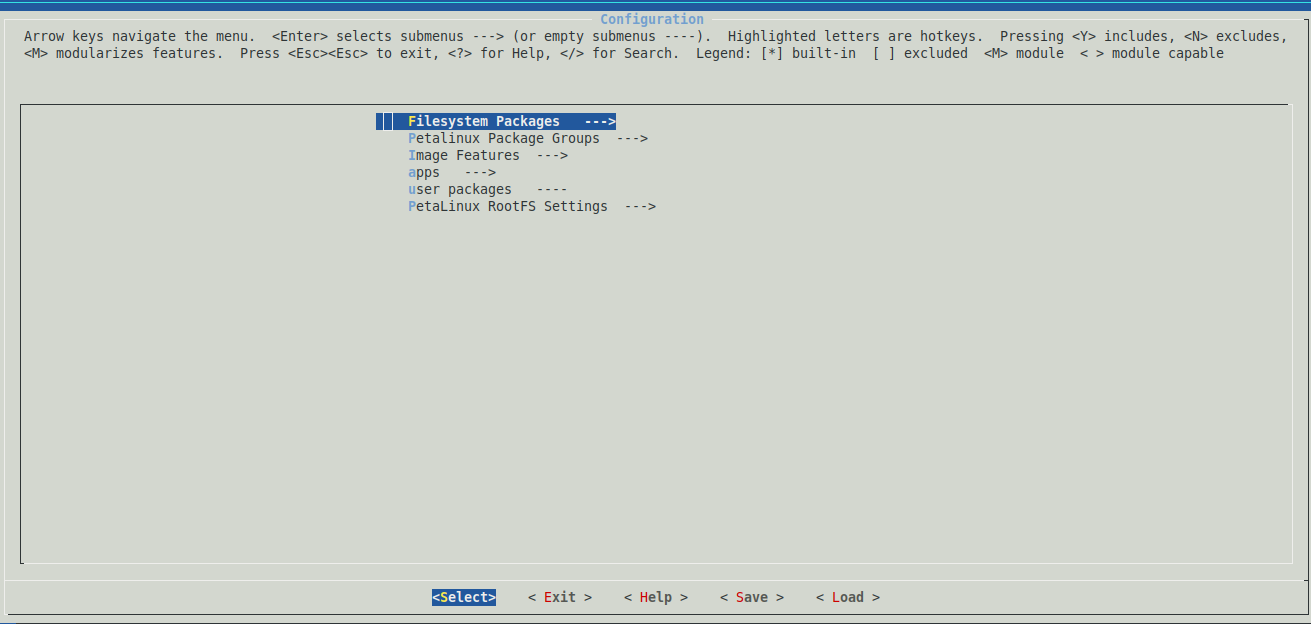
\includegraphics[width=\textwidth]{../images/fig/peta1.png}
\caption{Minh hoạ petalinux rootfs config terminal}
\label{fig:peta1}%
\end{figure}

Lưu lại và thoát
\item Vì ta boot bằng SD card, gõ lệnh:
 \begin{lst} 
 $ petallinux-config
 \end{lst} 
 Chọn Image Packaging Configuration > Root filesystem type (SD card) > SD card, nếu không thì file .ub sẽ vượt quá size của SD card.
 
\begin{figure}[H]
\centering
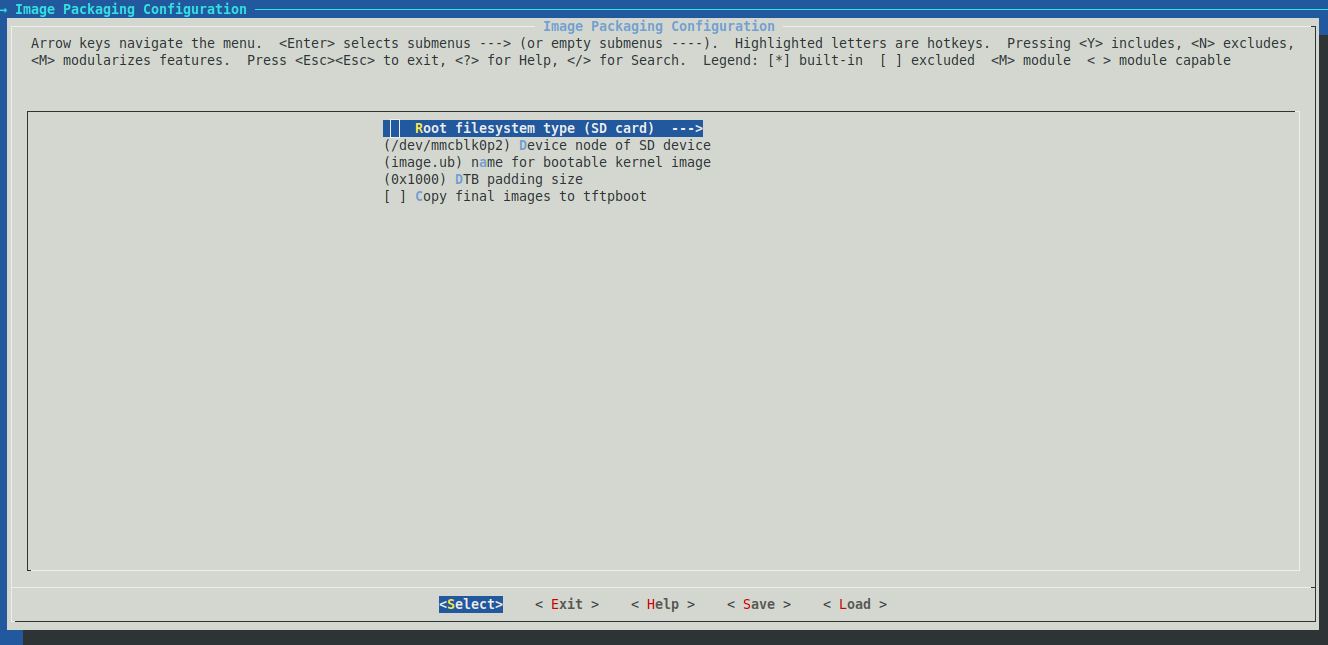
\includegraphics[width=\textwidth]{../images/fig/peta2.png}
\caption{Minh hoạ petalinux config terminal}
\label{fig:peta2}%
\end{figure}

\item Cuối cùng, build project
\begin{lst}
$ petalinux-build
\end{lst}
Kết quả sẽ được lưu vào thư mục images/linux/
\end{enumerate}
Tài liệu tham khảo thêm ở \cite{peta1, peta2, peta3, peta4}
\section{Tạo bootable SD Card}
\label{section:sdcard}
\subsection{Format SD card}
Format SD card thành 2 vùng, có thể dùng gparted hoặc fdisk:
\begin{enumerate}
\item \textbf{Free Space (MiB)}: 4, \textbf{New Size} (MiB) : 512, \textbf{File System} : FAT32, \textbf{Label} : BOOT
\item \textbf{Free Space (MiB)}: 0, Free Space Following(MiB): 0, \textbf{File System} : ext4, \textbf{Label} : rootfs
\end{enumerate}
\subsection{Tạo và chép các file cần thiết}
\begin{enumerate}
\item BOOT.BIN: Tạo file boot.bin với lệnh sau, lưu ý enviroment của petalinux
\begin{lst}
$ petalinux-package\
--boot\ 
--fpga <path_to_petalinux_project>/images/linux/system.bit\
--fsbl <path_to_petalinux_project>/images/linux/zynq_fsbl.elf \
--u-boot <path_to_petalinux_project>/images/linux/u-boot.elf
\end{lst}

\item Sau khi tạo xong, copy BOOT.BIN và image.ub, system.dtb (tìm trong <path_to_petalinux_project>/images/linux/) vào thư mục BOOT của SD card.
\item Giải nén thư mục rootfs.tar.gz trong <path_to_petalinux_project>/images/linux/ vào thư mục rootfs của SD card (lưu ý sử dụng quyền root)

\item Điều chỉnh zedboard vào chế độ boot bằng sd card (đặt jumper như hình, lắp sd card vào và tiến hành boot. Nếu board không tự boot thì gõ lệnh boot khi truy cập bằng UART.
 \begin{figure}[H]
\centering
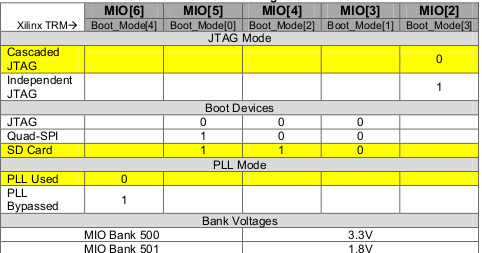
\includegraphics[width=.6\textwidth]{../images/fig/sd1.png}
\caption{ZedBoard Configuration Modes}
\label{fig:sd1}%
\end{figure}
Tài liệu tham khảo thêm ở \cite{sd1, sd2, sd3, sd4, sd5}
\end{enumerate}

\section{Build và Debug C++ OpenCV project}
\label{sdkguide}
Những hướng dẫn dưới đây giả sử máy tính đã được cài đặt Xilinx SDK, Zedboard đã boot thành công Petalinux và config eth0 cùng lớp mạng với máy tính.
\subsection*{Clone rootfs}
Để tạo một môi trường giống với Petalinux đã build trên zedboard, giải nén rootfs.tar.gz của petalinux vào một thư mục, tạm gọi là thư mục ROOTFS (lưu ý dùng quyền root để giải nén), xem hình \ref{fig:sdk1}1

\begin{figure}[H]
\centering
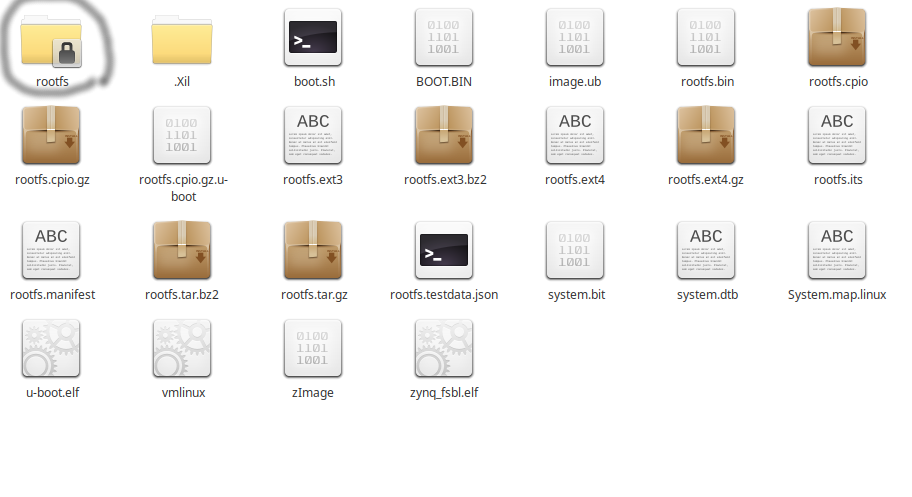
\includegraphics[width=.7\textwidth]{../images/fig/sdk1.png}
\caption{Thư mục rootfs}
\label{fig:sdk1}%
\end{figure}

\subsection*{Tạo project}
Vào XSDK, tạo một application project mới, chọn platform là Linux, language C++

\begin{figure}[H]
\centering
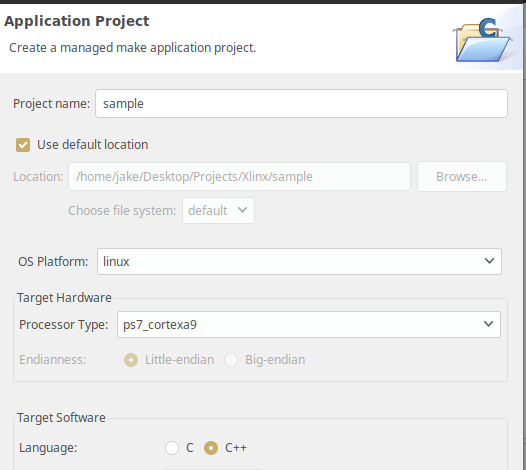
\includegraphics[width=.7\textwidth]{../images/fig/sdk2.png}
\caption{Tạo C++ OpenCV on Linux cortexa 9 processor application project}
\label{fig:sdk2}
\end{figure}

\subsection*{Setting C/C++ build trong XilinxSDK}
Để sử dụng thư viện OpenCV, ở project vừa tạo, chọn C/C++ build settings, thực hiện
\begin{itemize}
\item Ở Tab g++ compiler -> Directories, thêm vào các đường dẫn đến thư viện trong thư mục rootfs (hình \ref{fig:sdk1}, cụ thể là ROOT/usr/include/ và ROOT/usr/include/opencv2

\begin{figure}[H]
\centering
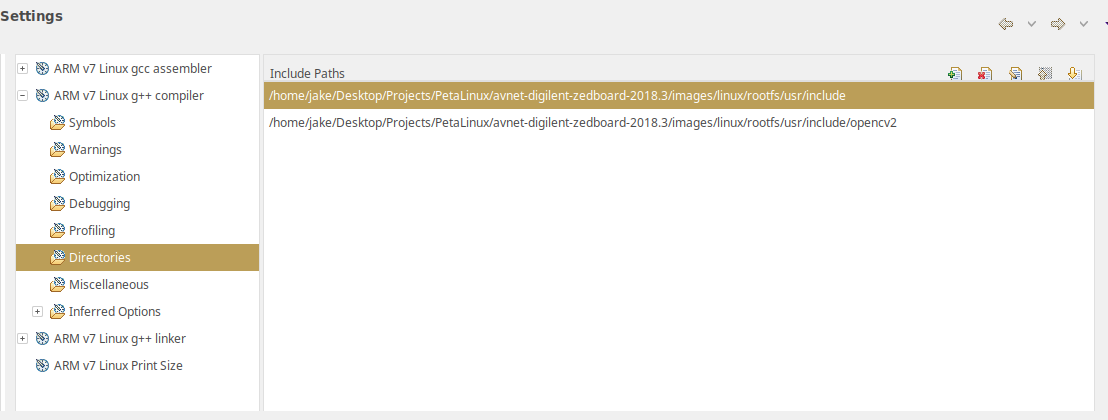
\includegraphics[width=.8\textwidth]{../images/fig/sdk3.png}
\caption{Điều chỉnh g++ compiler setting}
\label{fig:sdk3}
\end{figure}

\item Ở Tab g++ linker -> Libraries, thêm vào các linker cần thiết khi build, và các lib path ROOT/usr/lib và ROOT/usr/lib

\begin{figure}[H]
\centering
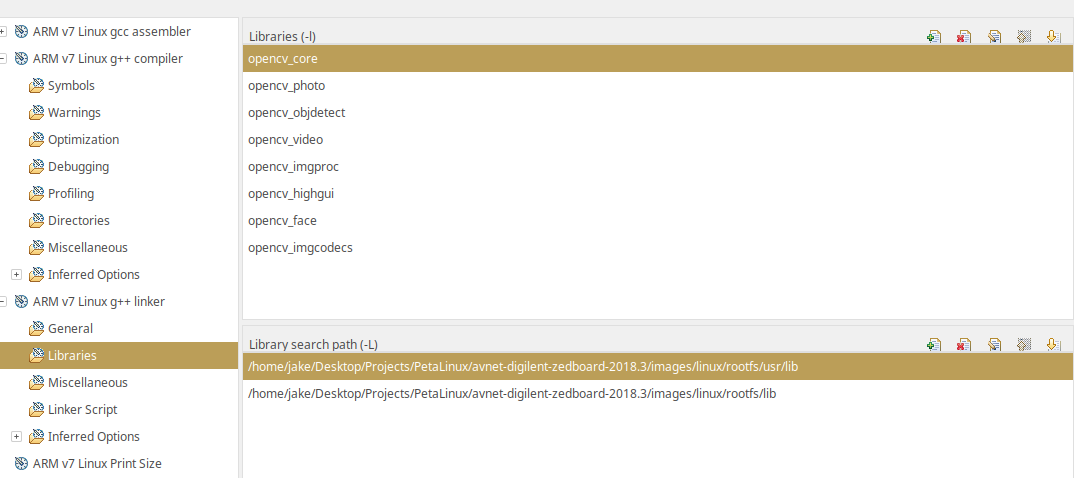
\includegraphics[width=.8\textwidth]{../images/fig/sdk4.png}
\caption{Điều chỉnh g++ linker libraries setting}
\label{fig:sdk4}
\end{figure}

\item Ở Tab g++ linker -> Miscellaneous, thêm vào dòng lệnh 

\begin{mdframed}[linecolor=black]
- -sysroot=ROOT
\end{mdframed} 


\begin{figure}[H]
\centering
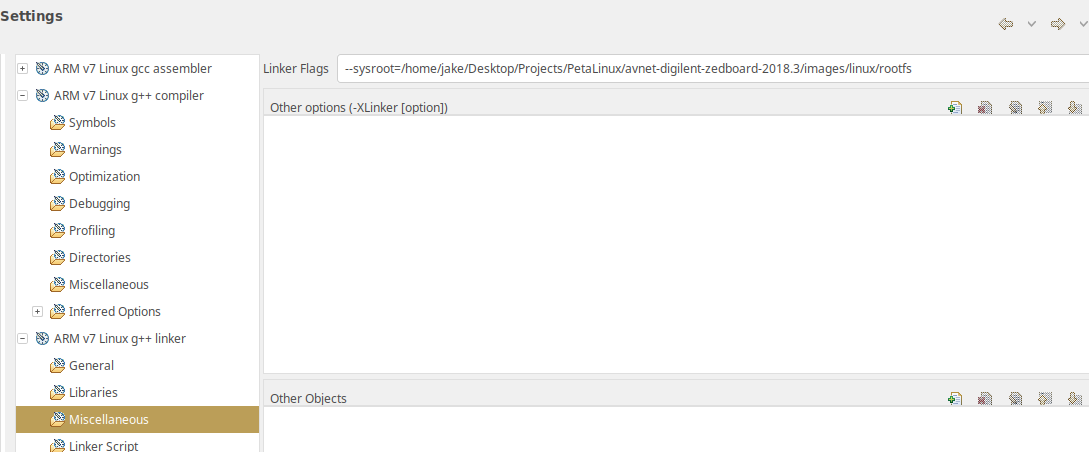
\includegraphics[width=.8\textwidth]{../images/fig/sdk5.png}
\caption{Điều chỉnh g++ linker miscellaneous setting}
\label{fig:sdk5}
\end{figure}

\item Để debug trên board thông qua linux agent, chọn Target connection > Linux TCF Agent, xem hình \ref{fig:sdk6}

\begin{figure}[H]
\centering
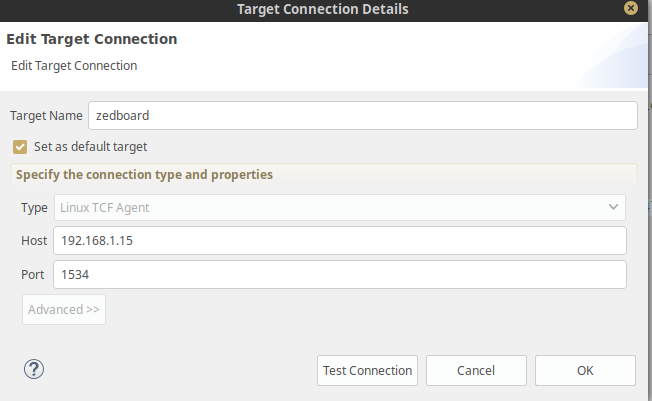
\includegraphics[width=.8\textwidth]{../images/fig/sdk6.png}
\caption{Cấu hình Linux TCF Agent}
\label{fig:sdk6}
\end{figure}
\end{itemize}
Tham khảo thêm tại \cite{sdk1, sdk2, sdk3}

\subsection*{Cross-compiler ffmpeg cho OpenCV trên ARM}
\label{ffmpeg}
Làm theo hướng dẫn ở \cite{ffmpeg1} để cross-compile thư mục local \par
Sau khi đã hoàn thành: 
\begin{enumerate}
\item Ở C/C++ Build Settings > Tab g++ compiler > Directories, thêm vào đường dẫn đến ROOT/usr/local/include vừa mới tạo
\item Ở C/C++ Build Settings > Tab g++ linker > Libraries, thêm vào đường dẫn đến ROOT/usr/local/lib
\item Thêm LD_LIBRARY_PATH = /usr/local/lib vào biến enviroment trong Run as > Run Configuration 
\end{enumerate}
%%%%%%%%%%%%%%%%%%%%%%%%%%%%%%%%%%%%%%%%%%%%%%%
\cleardoublepage
\section{Phụ lục khác}
\listoffigures
\listoftables

%%%%----Phụ lục----------
\cleardoublepage
\bibliography{thamkhao} 
\bibliographystyle{ieeetr}
\end{document}

